\section{各サブシステムのフローチャート}
各サブシステムのフローチャートを示します。

\subsection{ログインシステム(学生側)}
学生側のログインシステムのシーケンス図とフローチャートを以下に示します。
\begin{figure}[htbp]
  \begin{center}
    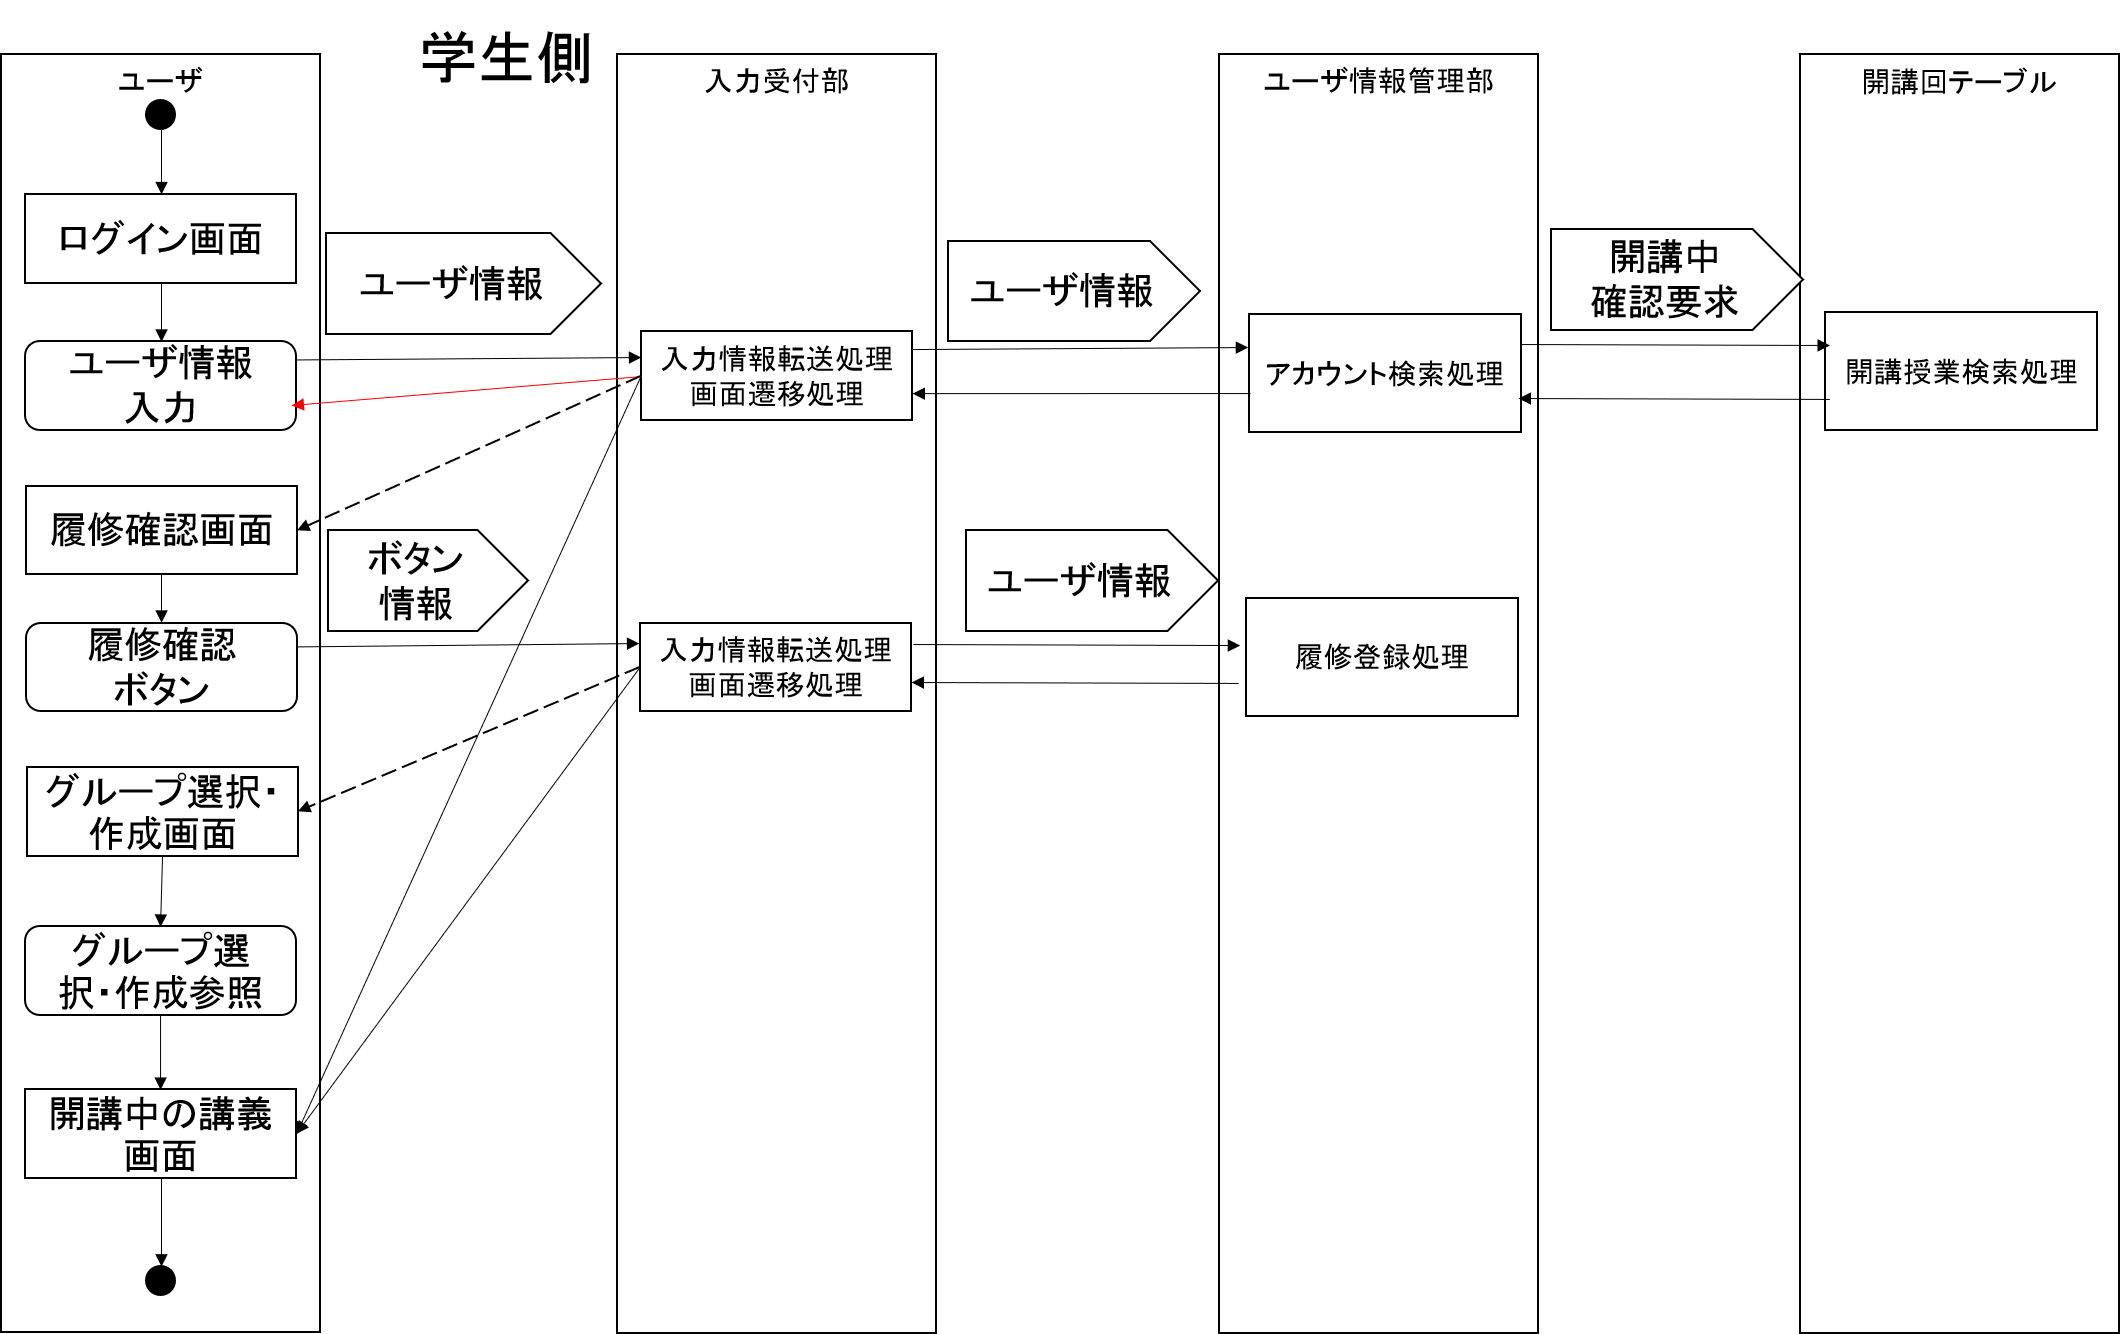
\includegraphics[width=1\linewidth,clip]{./img/login/main.png}
    \caption{ログインシステム(学生側)のシーケンス図}\label{fig:loginseaquence}
  \end{center}
\end{figure}

\begin{figure}[htbp]
  \begin{center}
    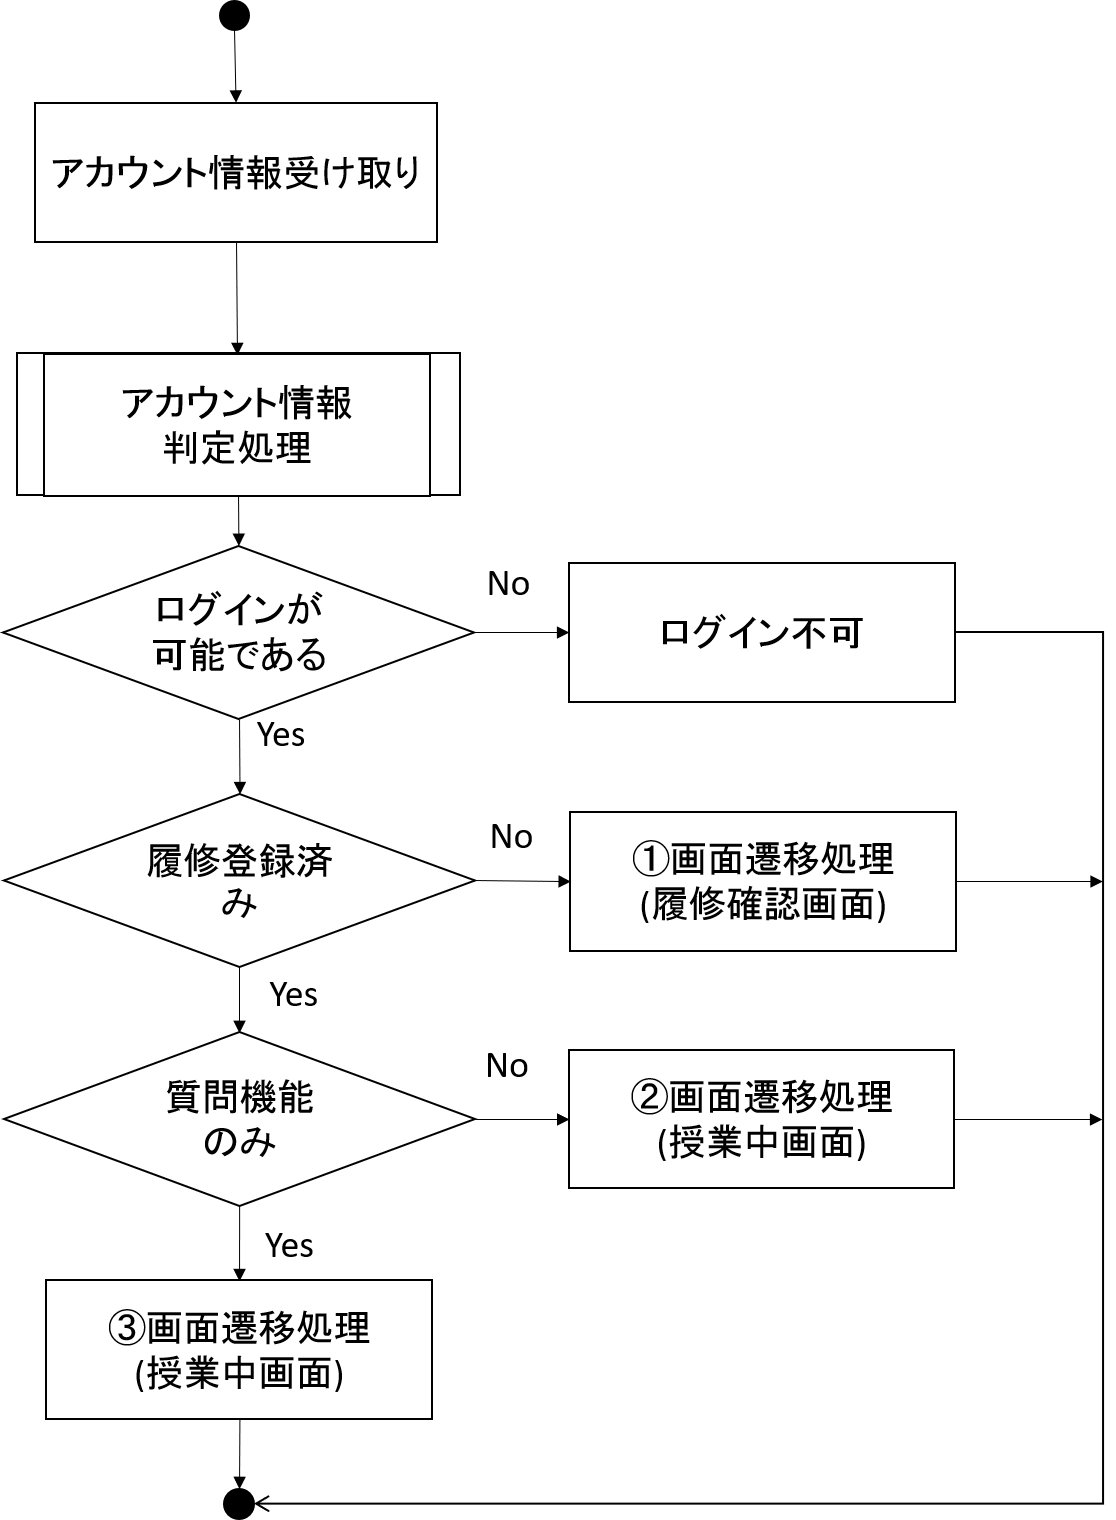
\includegraphics[width=0.5\linewidth,clip]{./img/login/sub1.png}
    \caption{[1]のフローチャート}\label{fig:loginflow0}
  \end{center}
\end{figure}


\begin{figure}[htbp]
 \begin{minipage}{0.5\hsize}
  \begin{center}
   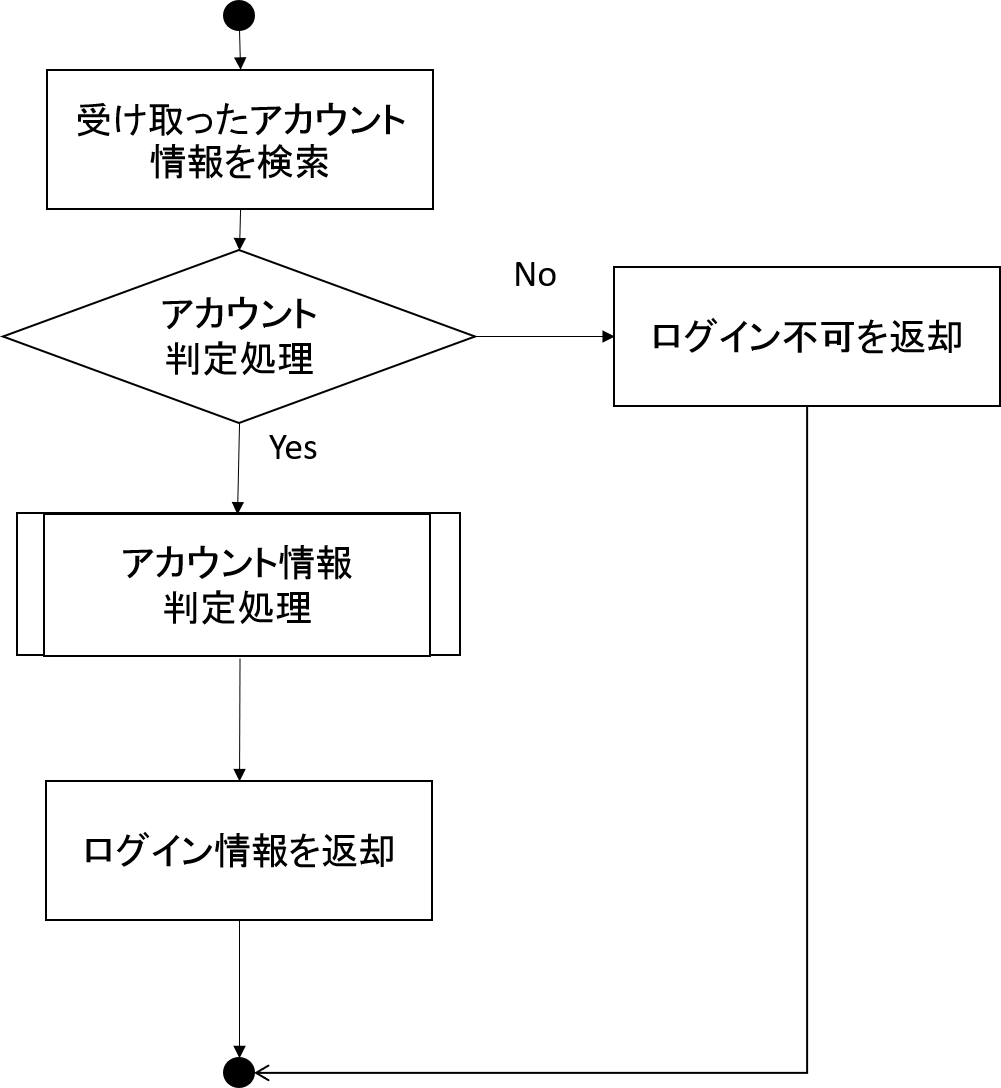
\includegraphics[width=1\linewidth,clip]{./img/login/sub2.png}
  \end{center}
 \end{minipage}
 \begin{minipage}{0.5\hsize}
  \begin{center}
   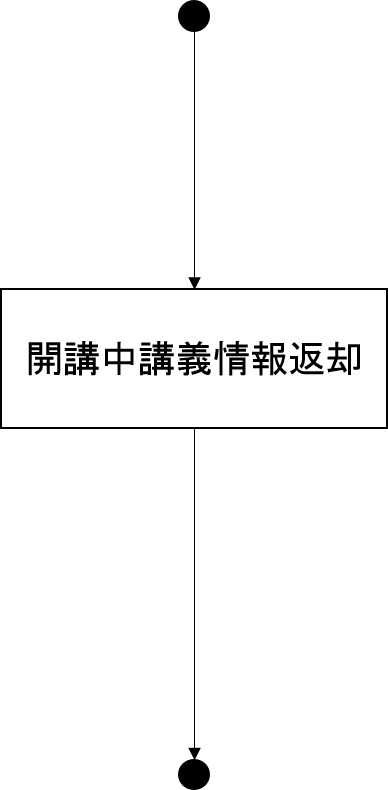
\includegraphics[width=0.5\linewidth,clip]{./img/login/sub3.png}
  \end{center}
 \end{minipage}
 \caption{左:[2]のフローチャート 右:[3]のフローチャート}\label{fig:loginflow1}
\end{figure}

\begin{figure}[htbp]
 \begin{minipage}{0.5\hsize}
  \begin{center}
   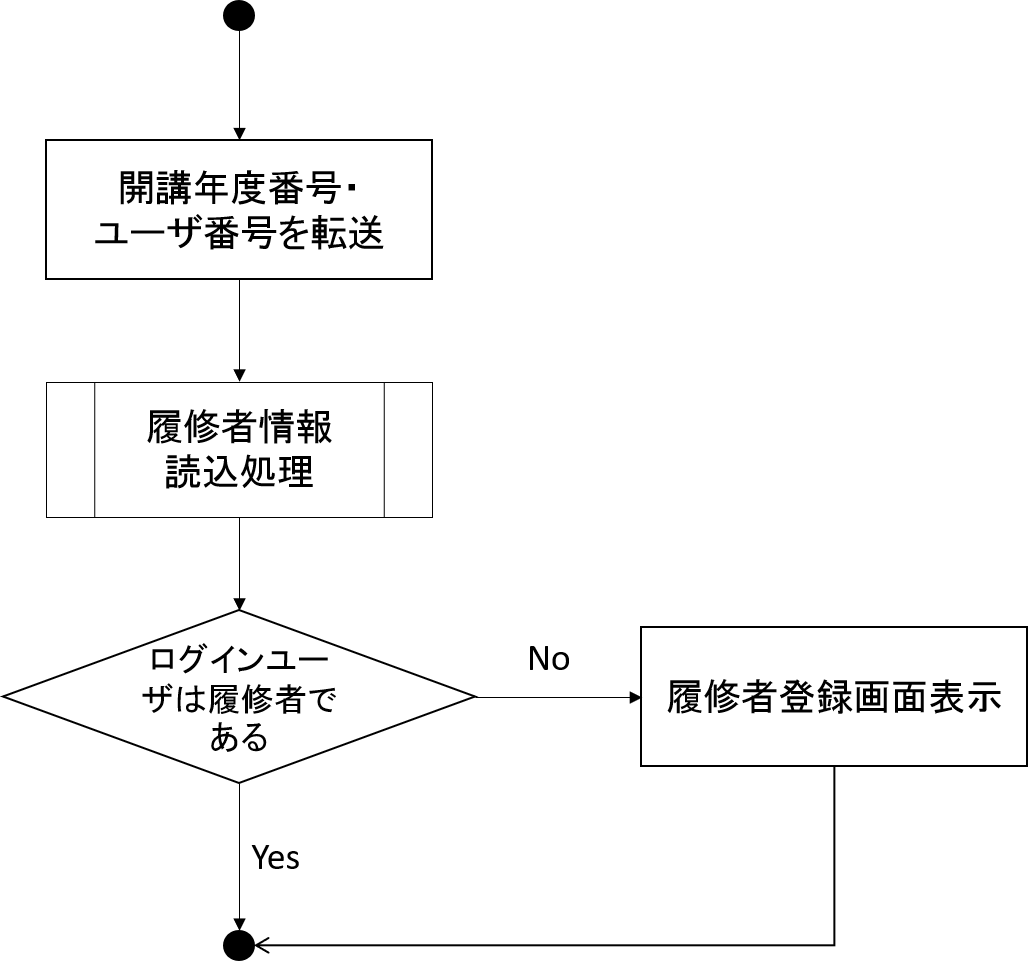
\includegraphics[width=1\linewidth,clip]{./img/login/sub4.png}
  \end{center}
 \end{minipage}
 \begin{minipage}{0.5\hsize}
  \begin{center}
   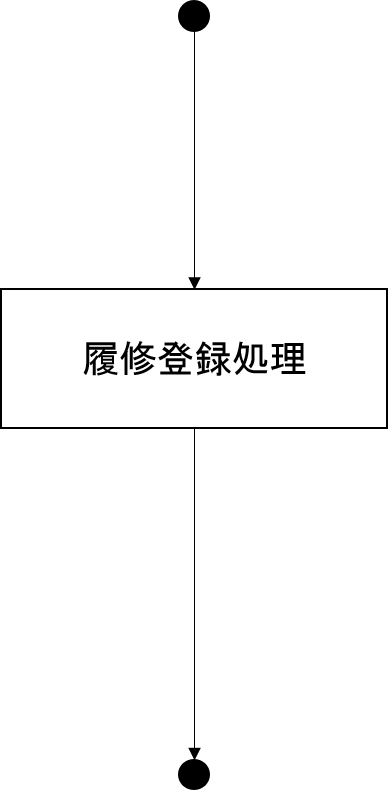
\includegraphics[width=0.5\linewidth,clip]{./img/login/sub5.png}
  \end{center}
 \end{minipage}
 \caption{左:[4]のフローチャート 右:[5]のフローチャート}\label{fig:loginflow2}
\end{figure}

\newpage

\subsection{ログインシステム(管理者側)}
管理者側のログインシステムのシーケンス図とフローチャートを以下に示します。

\begin{figure}[htbp]
  \begin{center}
    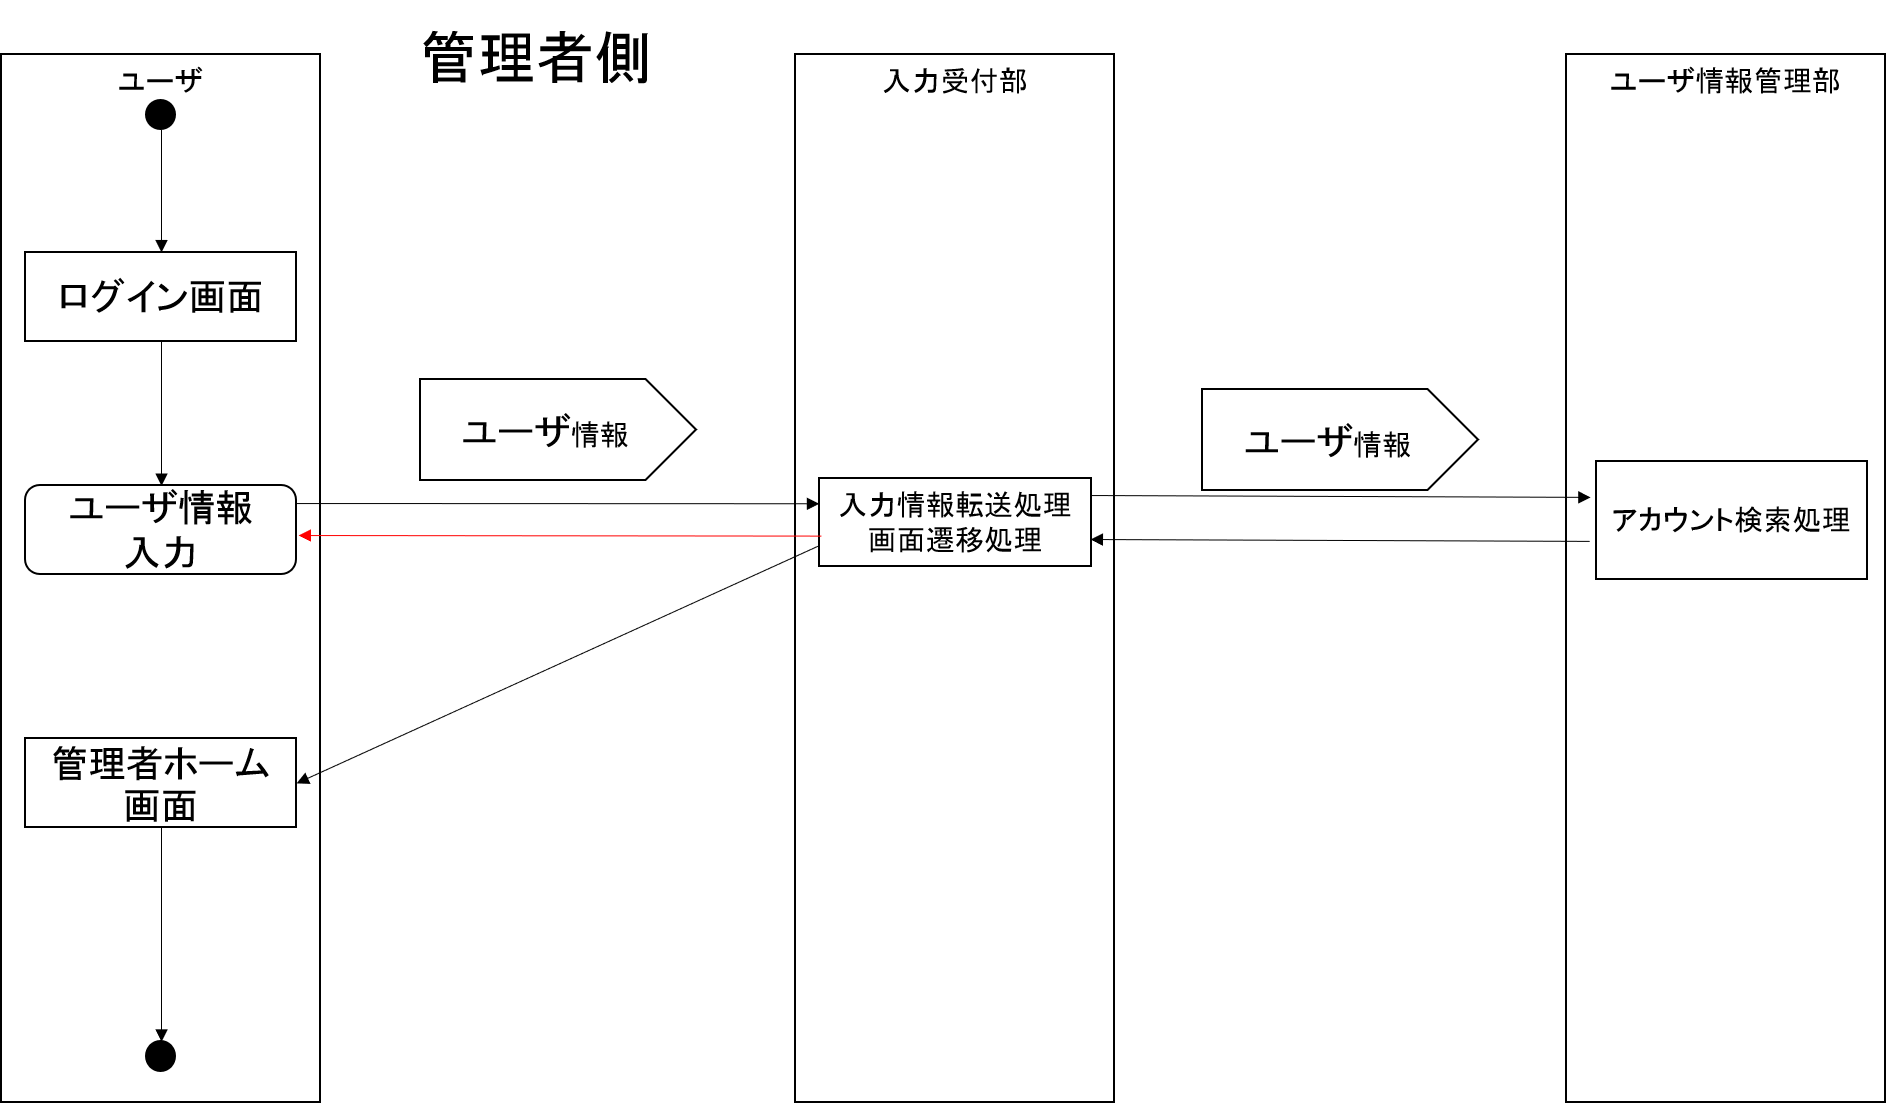
\includegraphics[width=1\linewidth,clip]{./img/admin_login/main.png}
    \caption{ログインシステム(管理者側)のシーケンス図}\label{fig:adminloginseaquence}
  \end{center}
\end{figure}


\begin{figure}[htbp]
 \begin{minipage}{0.5\hsize}
  \begin{center}
   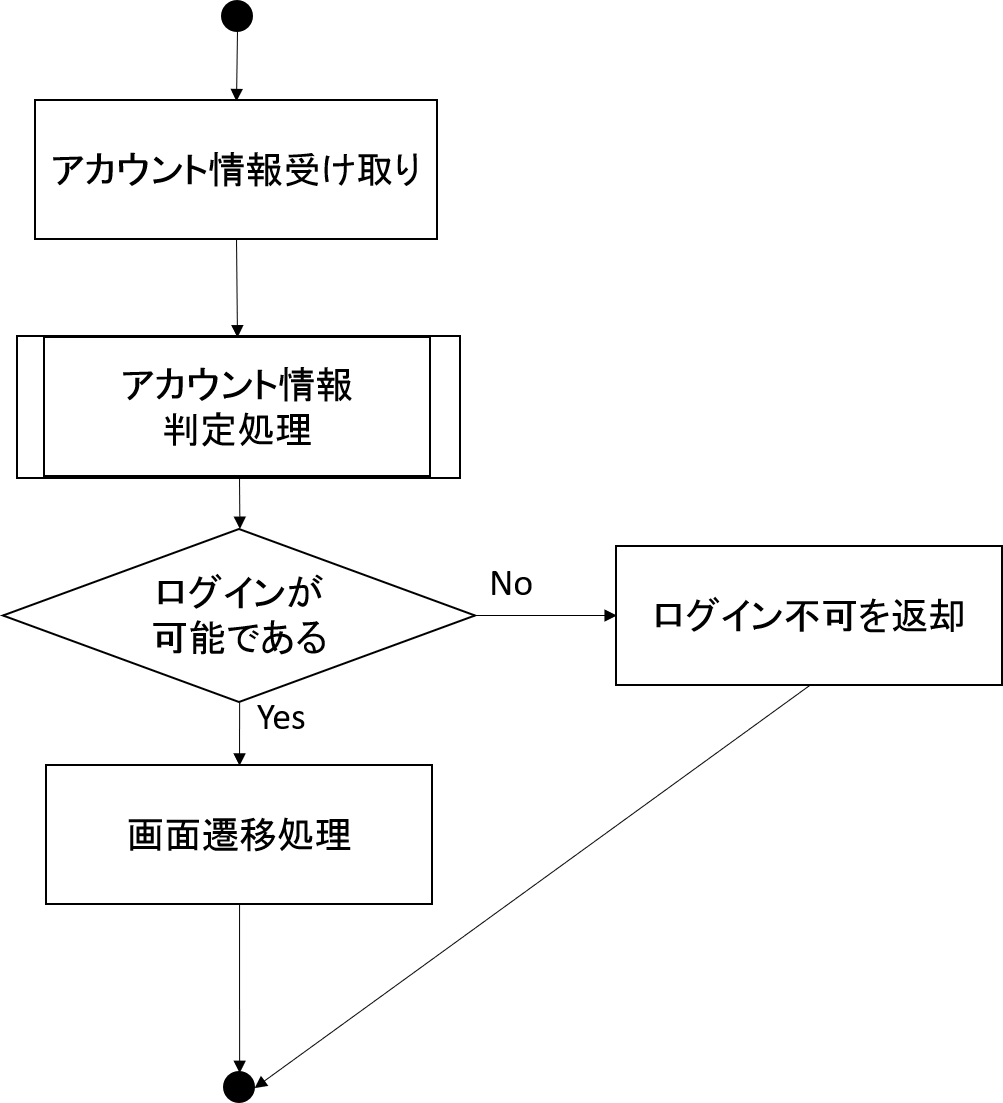
\includegraphics[width=1\linewidth,clip]{./img/admin_login/sub1.png}
  \end{center}
 \end{minipage}
 \begin{minipage}{0.5\hsize}
  \begin{center}
   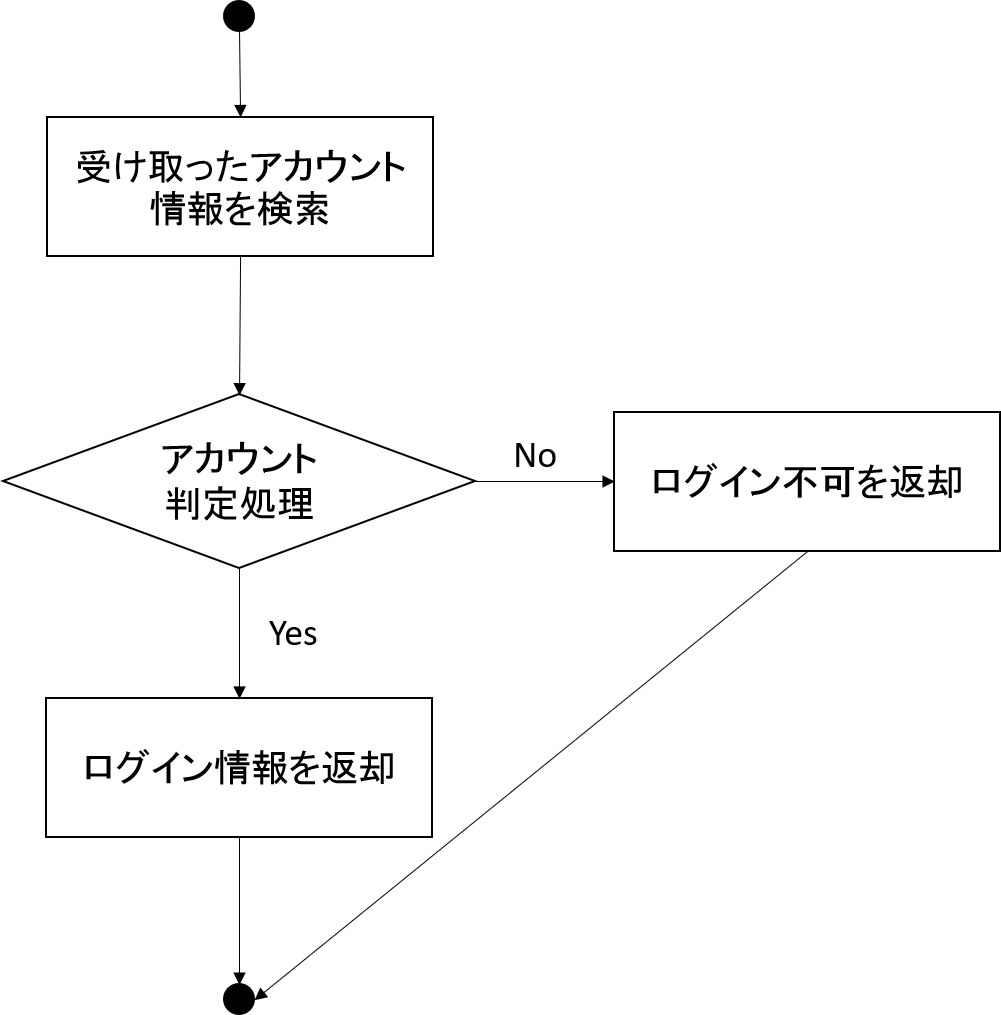
\includegraphics[width=1\linewidth,clip]{./img/admin_login/sub2.png}
  \end{center}
 \end{minipage}
 \caption{左:[1]のフローチャート 右:[2]のフローチャート}\label{fig:adminloginflow0}
\end{figure}

\newpage
\subsection{アカウント作成システム(学生側)}
学生側のアカウント作成システムのシーケンス図とフローチャートを以下に示します。

\begin{figure}[htbp]
  \begin{center}
    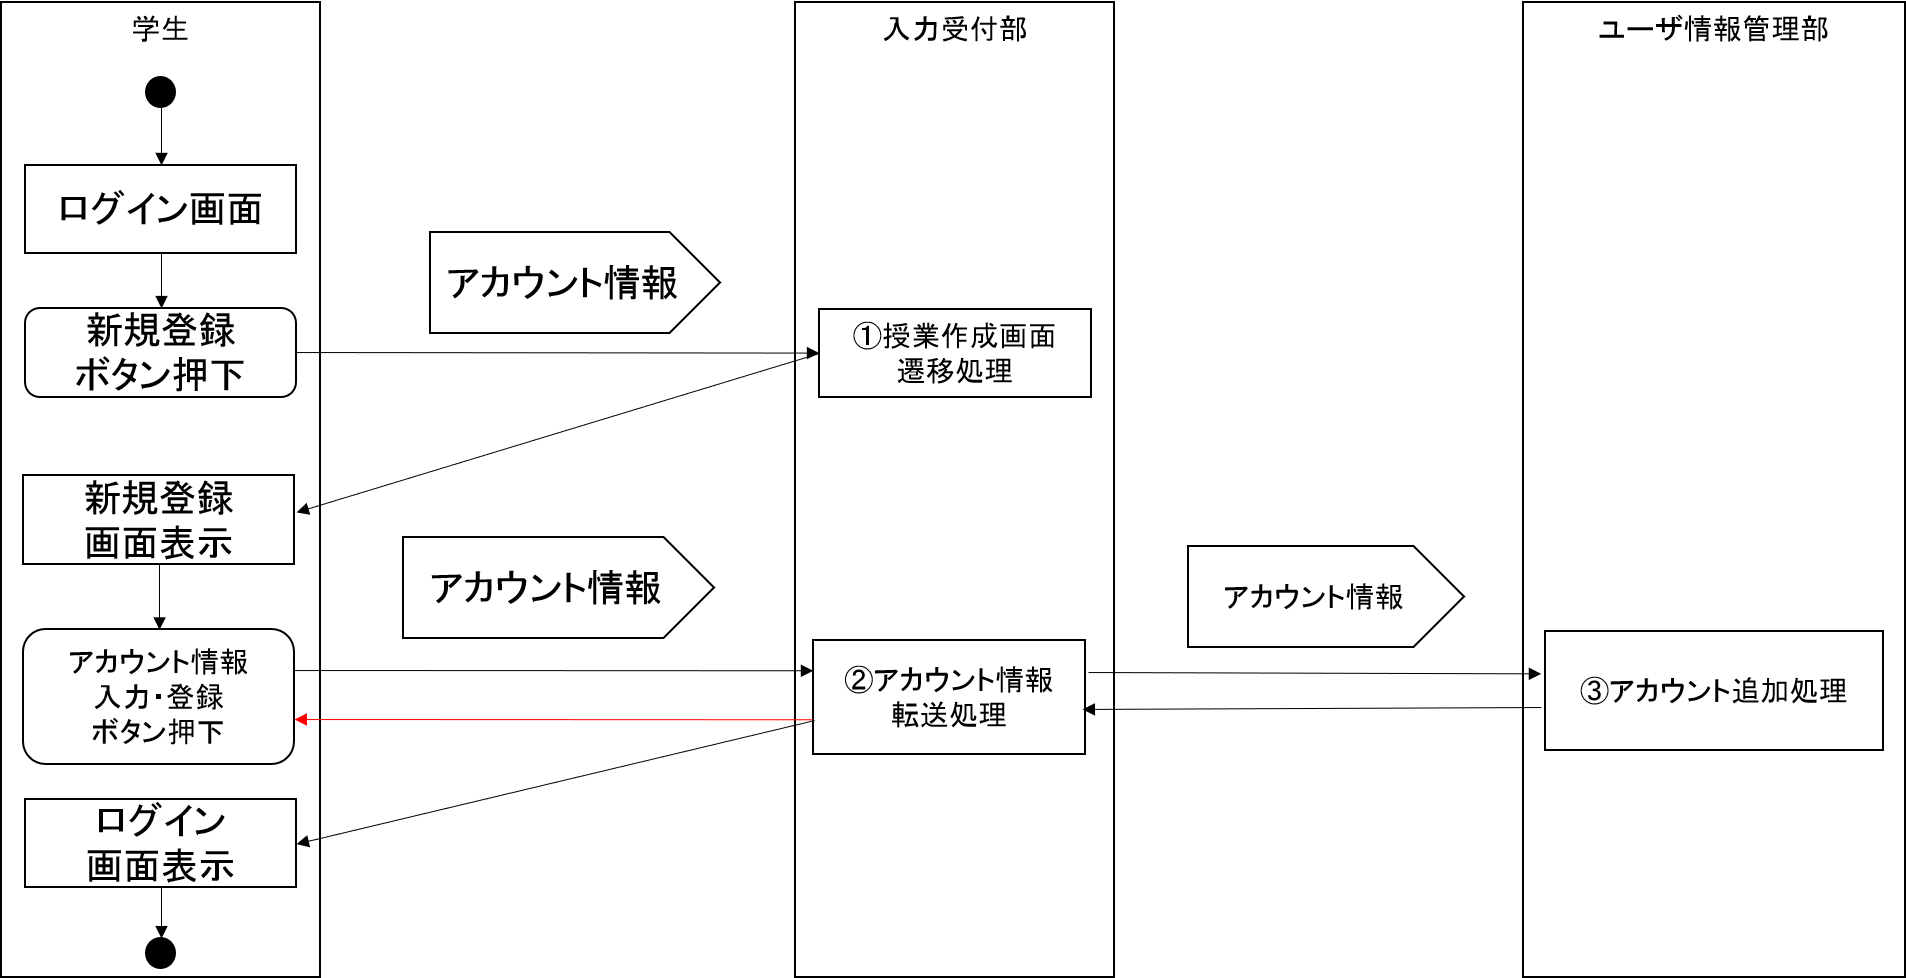
\includegraphics[width=1\linewidth,clip]{./img/create_account/main.png}
    \caption{アカウント作成システム(学生側)のシーケンス図}\label{fig:createseaquence}
  \end{center}
\end{figure}

\begin{figure}[htbp]
 \begin{minipage}{0.5\hsize}
  \begin{center}
   \includegraphics[width=0.5\linewidth,clip]{./img/create_account/sub1.png}
  \end{center}
 \end{minipage}
 \begin{minipage}{0.5\hsize}
  \begin{center}
   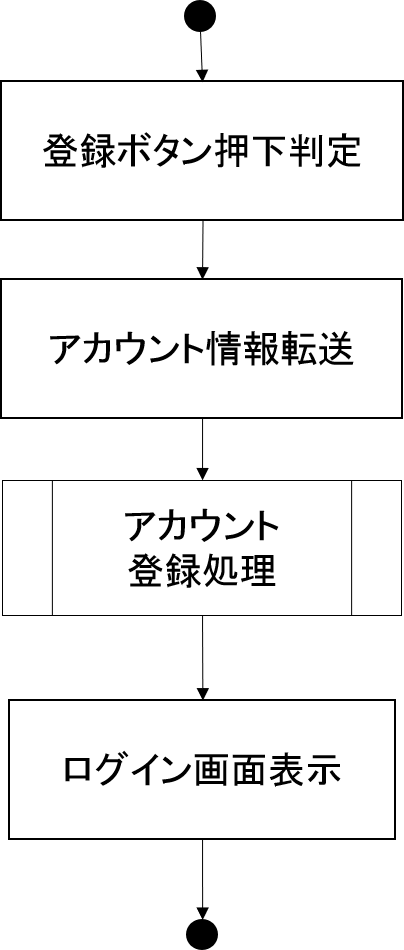
\includegraphics[width=1\linewidth,clip]{./img/create_account/sub2.png}
  \end{center}
 \end{minipage}
 \caption{左:[1]のフローチャート 右:[2]のフローチャート}\label{fig:createaccountflow0}
\end{figure}

\begin{figure}[htbp]
  \begin{center}
    \includegraphics[width=0.5\linewidth,clip]{./img/create_account/sub3.png}
    \caption{[3]のフローチャート}\label{fig:createaccountflow1}
  \end{center}
\end{figure}

\newpage
\subsection{アカウント作成システム(管理者側)}
管理者側のアカウント作成システムのシーケンス図とフローチャートを以下に示します。

\begin{figure}[htbp]
  \begin{center}
    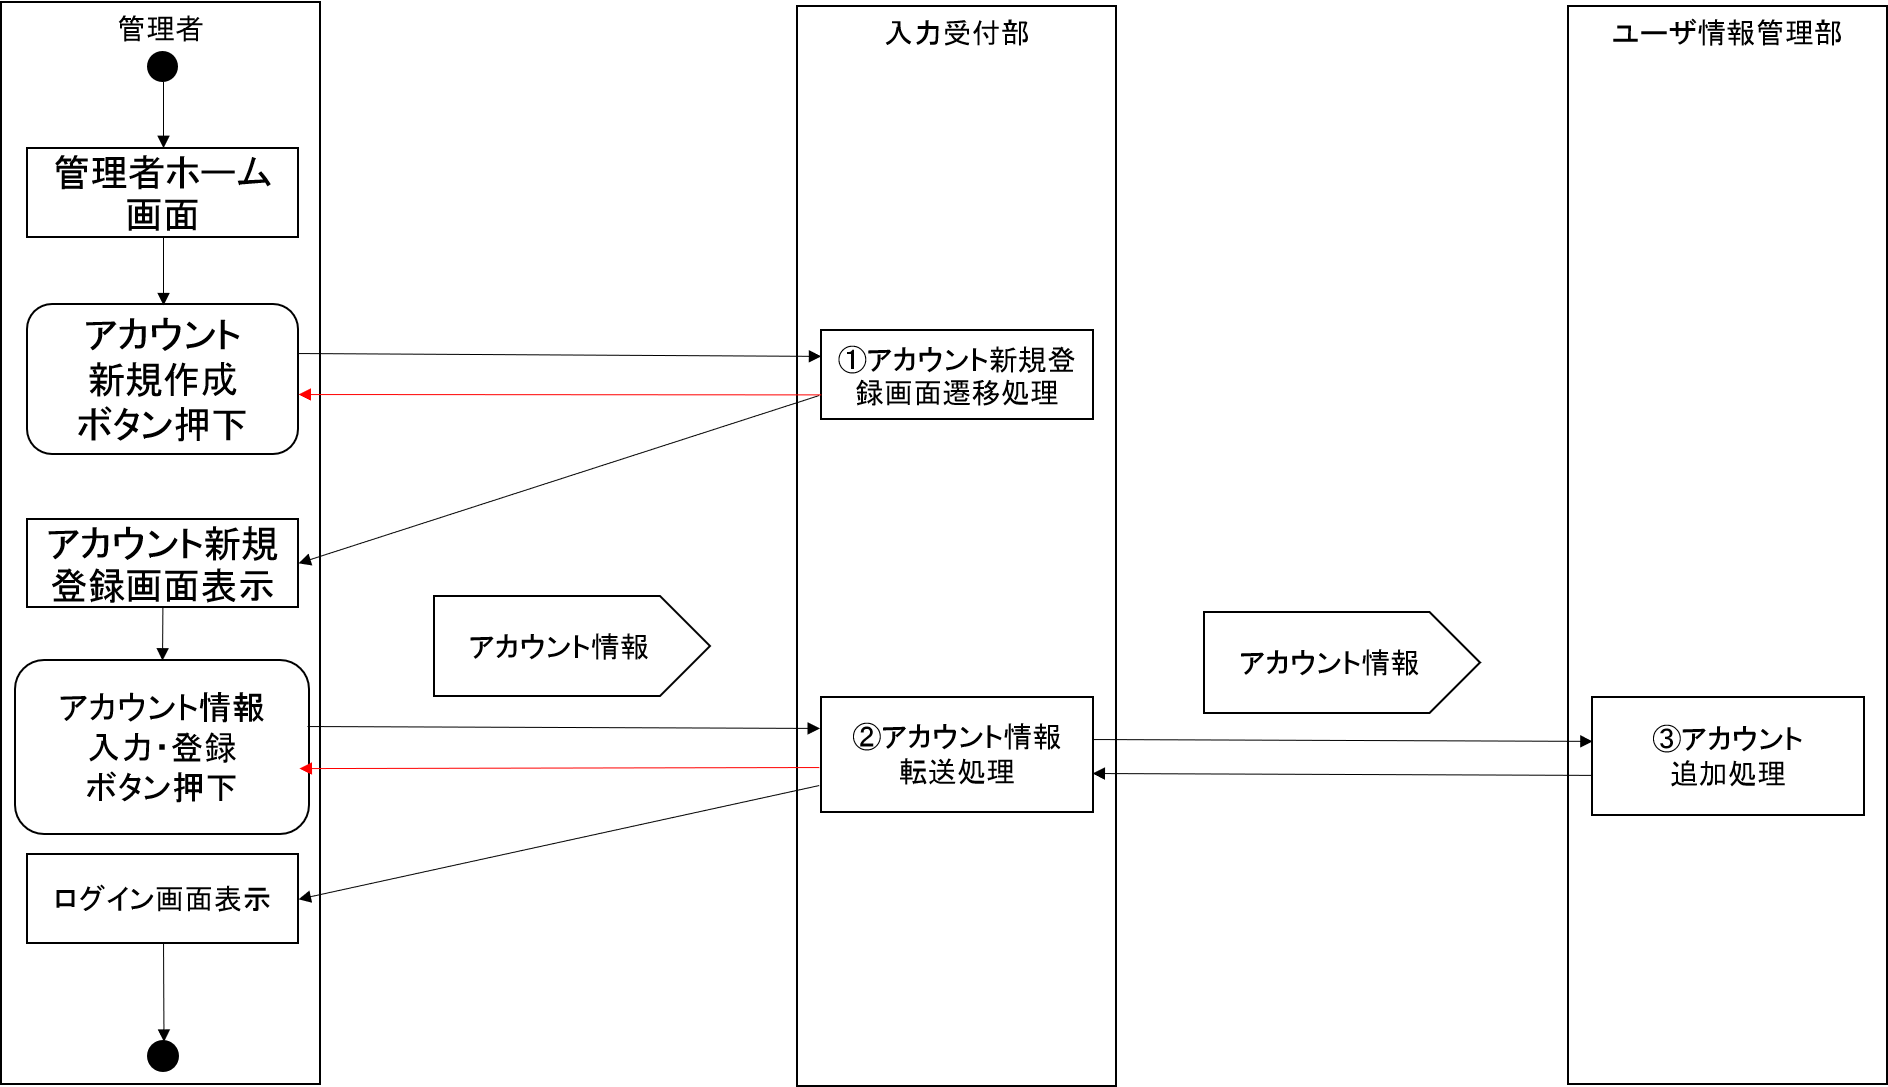
\includegraphics[width=1\linewidth,clip]{./img/admin_create_account/main.png}
    \caption{アカウント作成システム(管理者側)のシーケンス図}\label{fig:admincreateseaquence}
  \end{center}
\end{figure}

\begin{figure}[htbp]
 \begin{minipage}{0.5\hsize}
  \begin{center}
   \includegraphics[width=0.5\linewidth,clip]{./img/admin_create_account/sub1.png}
  \end{center}
 \end{minipage}
 \begin{minipage}{0.5\hsize}
  \begin{center}
   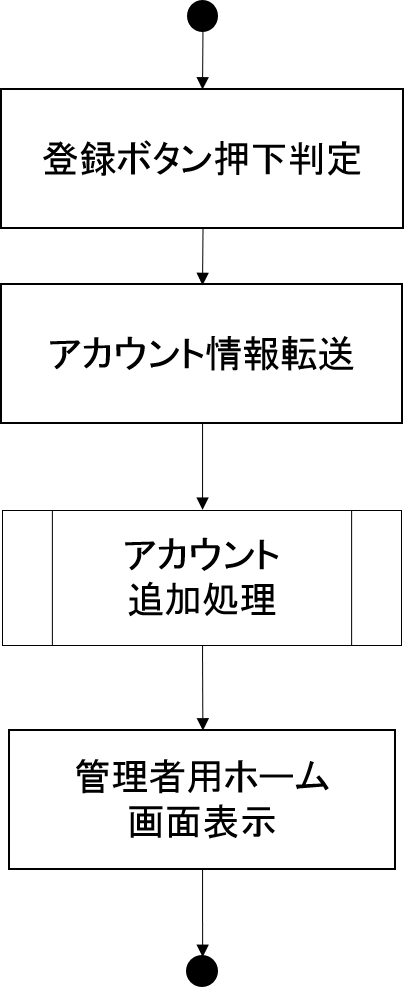
\includegraphics[width=1\linewidth,clip]{./img/admin_create_account/sub2.png}
  \end{center}
 \end{minipage}
 \caption{左:[1]のフローチャート 右:[2]のフローチャート}\label{fig:admincreateaccountflow0}
\end{figure}

\begin{figure}[htbp]
  \begin{center}
    \includegraphics[width=0.5\linewidth,clip]{./img/admin_create_account/sub3.png}
    \caption{[3]のフローチャート}\label{fig:admincreateaccountflow1}
  \end{center}
\end{figure}


\newpage
\subsection{アカウント情報編集システム}
アカウント情報編集システムのシーケンス図とフローチャートを以下に示します。

\begin{figure}[htbp]
  \begin{center}
    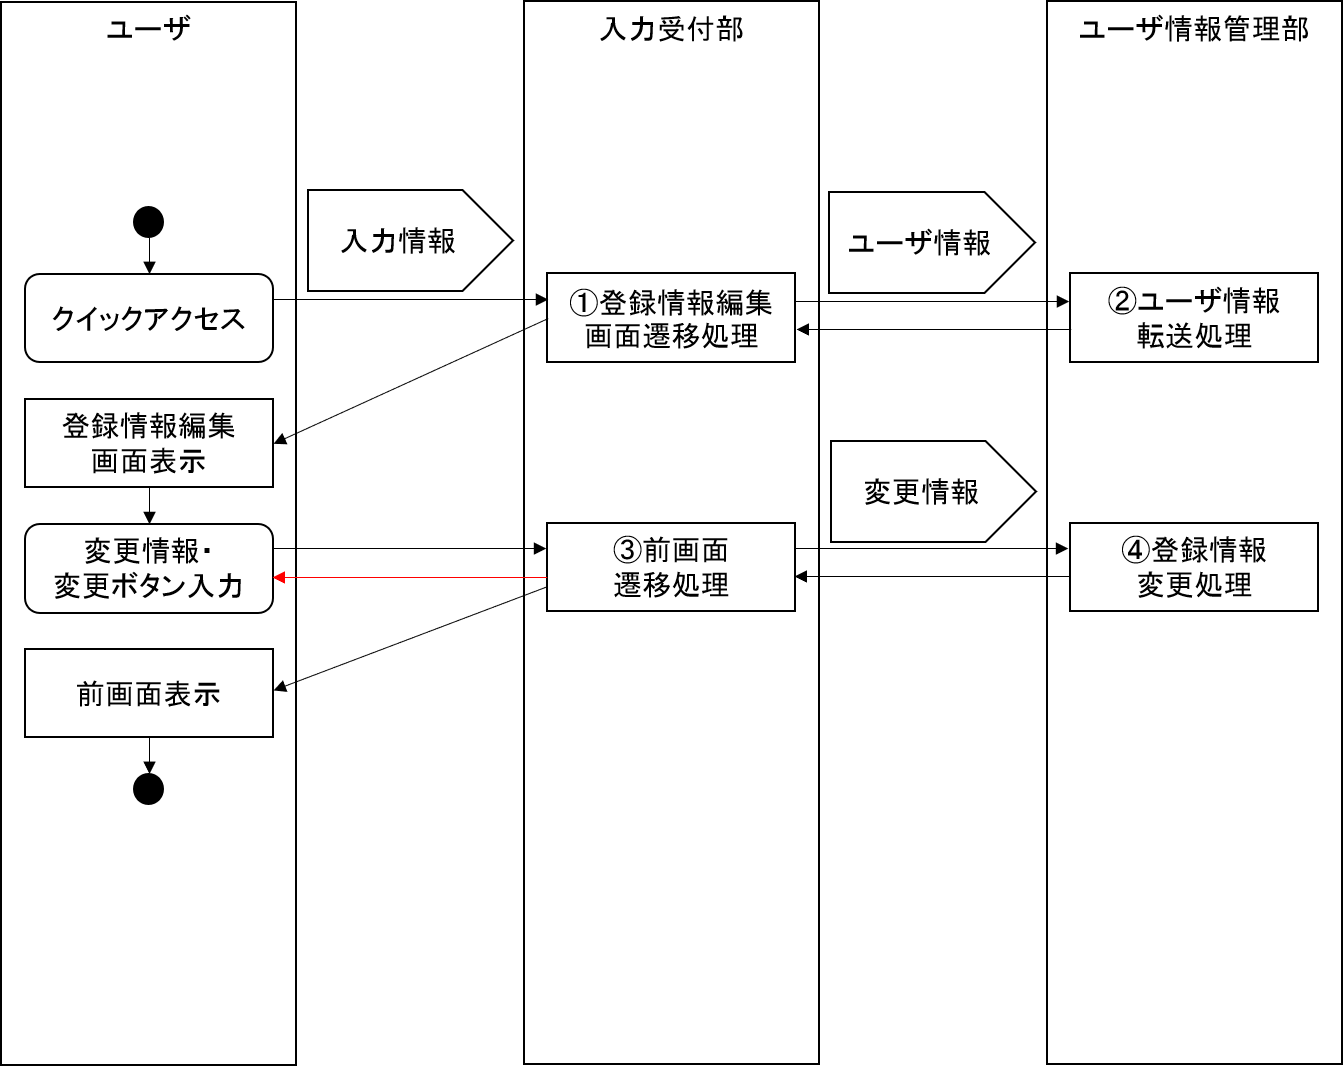
\includegraphics[width=1\linewidth,clip]{./img/edit_account/main.png}
    \caption{アカウント情報編集システムのシーケンス図}\label{fig:editaccountseaquence}
  \end{center}
\end{figure}

\begin{figure}[htbp]
 \begin{minipage}{0.5\hsize}
  \begin{center}
   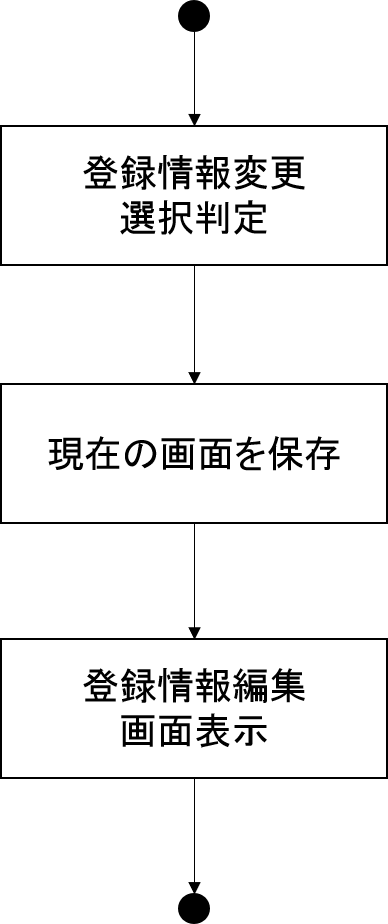
\includegraphics[width=0.5\linewidth,clip]{./img/edit_account/sub1.png}
  \end{center}
 \end{minipage}
 \begin{minipage}{0.5\hsize}
  \begin{center}
   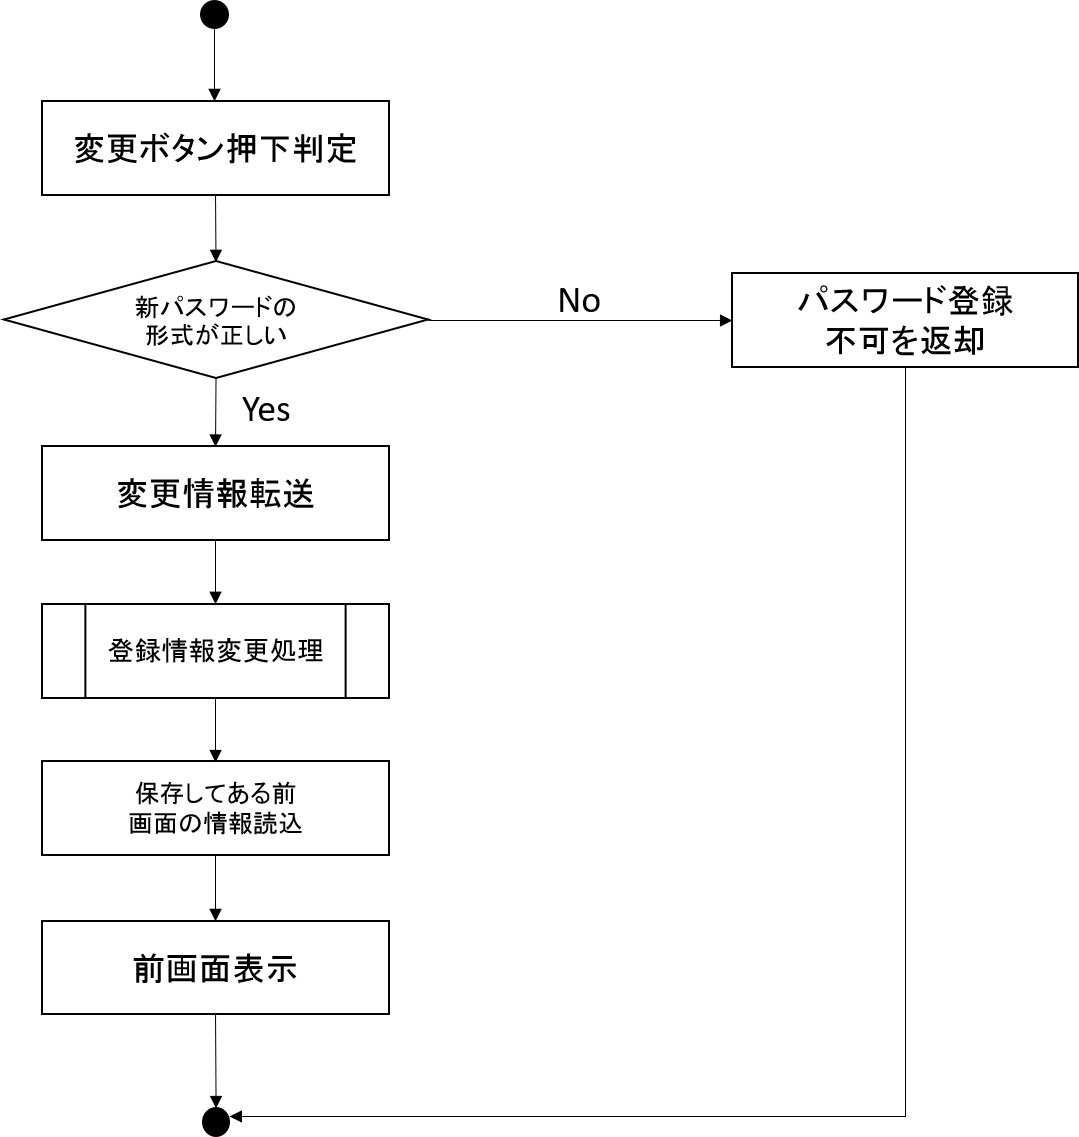
\includegraphics[width=0.5\linewidth,clip]{./img/edit_account/sub2.png}
  \end{center}
 \end{minipage}
 \caption{左:[1]のフローチャート 右:[2]のフローチャート}\label{fig:editaccountflow0}
\end{figure}

\begin{figure}[htbp]
 \begin{minipage}{0.5\hsize}
  \begin{center}
   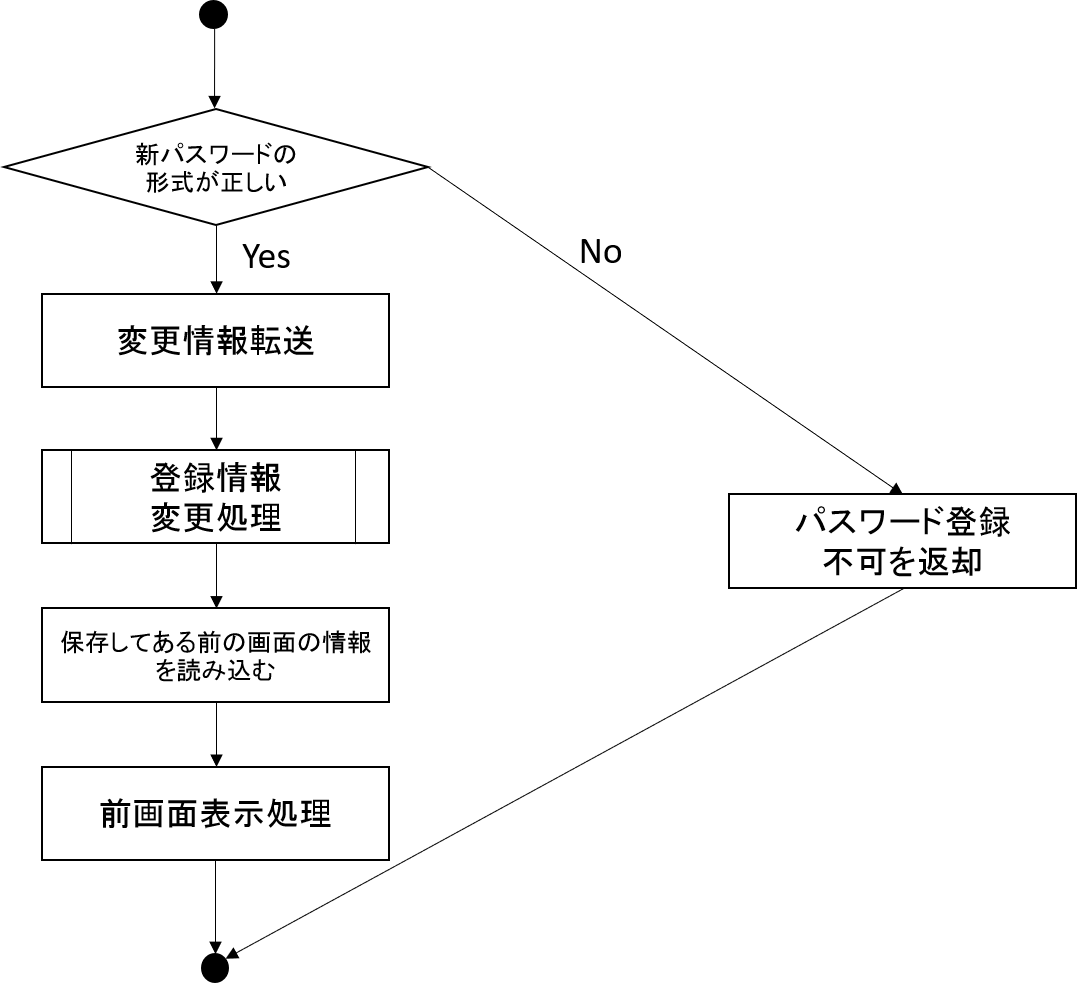
\includegraphics[width=1\linewidth,clip]{./img/edit_account/sub3.png}
  \end{center}
 \end{minipage}
 \begin{minipage}{0.5\hsize}
  \begin{center}
   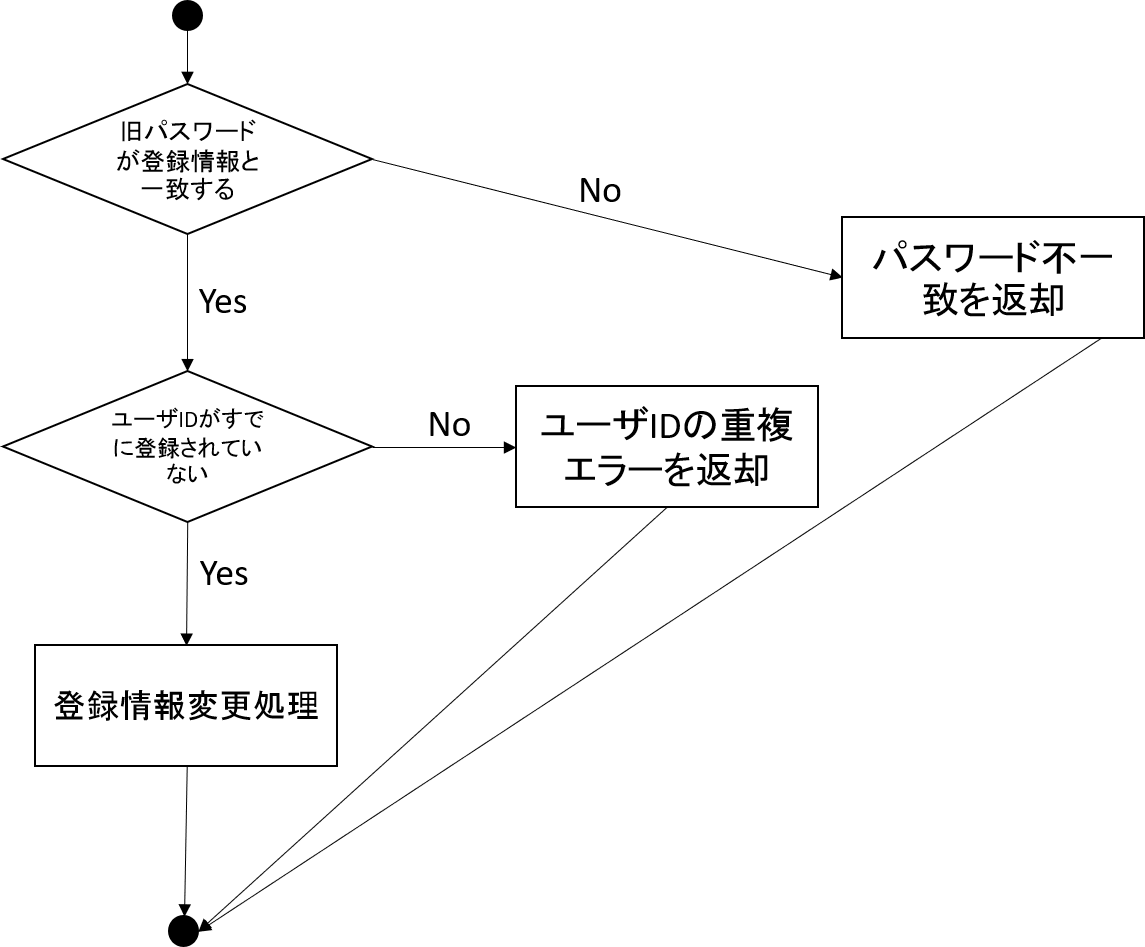
\includegraphics[width=1\linewidth,clip]{./img/edit_account/sub4.png}
  \end{center}
 \end{minipage}
 \caption{左:[3]のフローチャート 右:[4]のフローチャート}\label{fig:editaccountflow0}
\end{figure}


\newpage
\subsection{グループ作成システム}
グループ作成システムのシーケンス図とフローチャートを以下に示します。

\begin{figure}[htbp]
  \begin{center}
    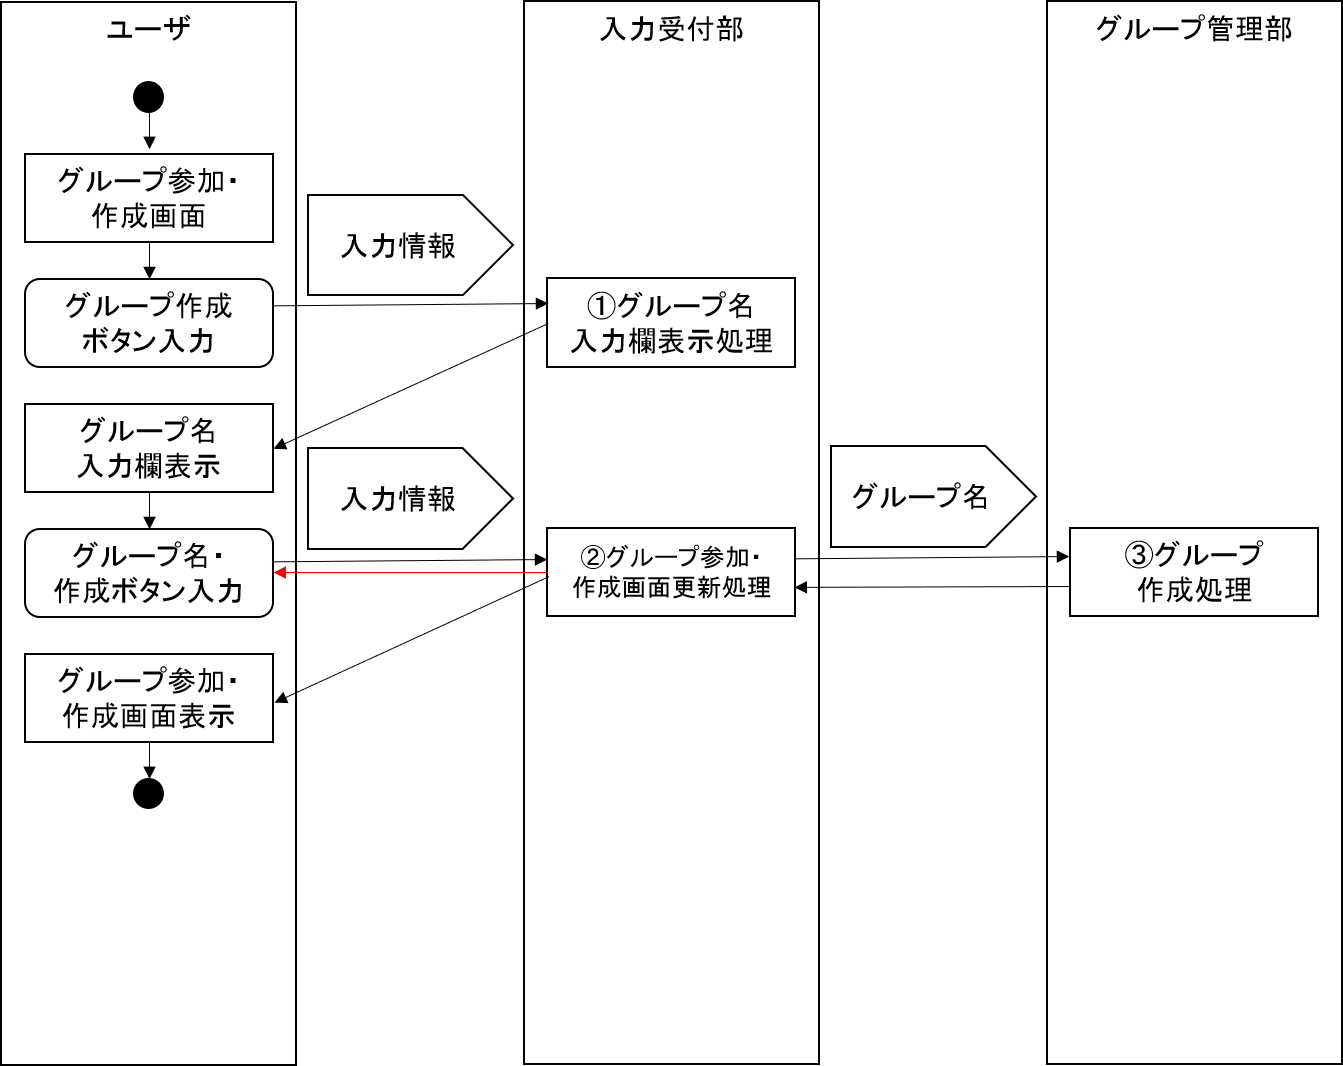
\includegraphics[width=1\linewidth,clip]{./img/create_group/main.png}
    \caption{グループ作成システムのシーケンス図}\label{fig:creategroupseaquence}
  \end{center}
\end{figure}

\begin{figure}[htbp]
 \begin{minipage}{0.5\hsize}
  \begin{center}
   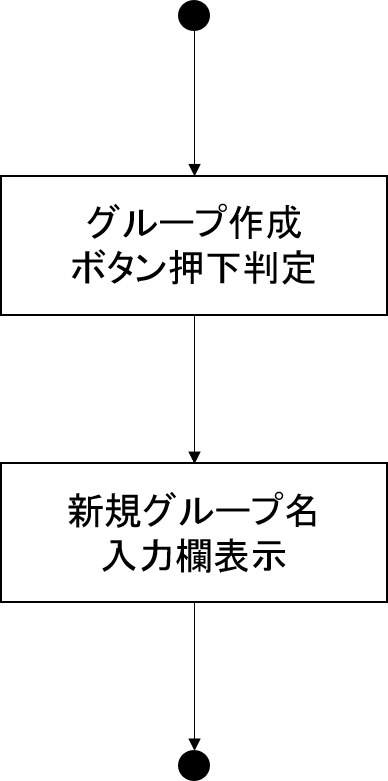
\includegraphics[width=0.5\linewidth,clip]{./img/create_group/sub1.png}
  \end{center}
 \end{minipage}
 \begin{minipage}{0.5\hsize}
  \begin{center}
   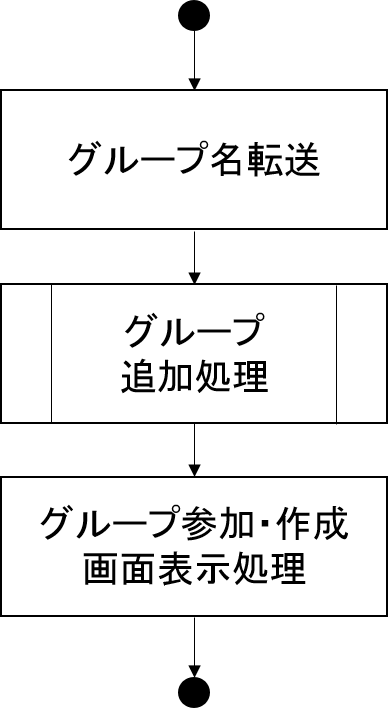
\includegraphics[width=0.5\linewidth,clip]{./img/create_group/sub2.png}
  \end{center}
 \end{minipage}
 \caption{左:[1]のフローチャート 右:[2]のフローチャート}\label{fig:creategroupflow0}
\end{figure}

\begin{figure}[htbp]
  \begin{center}
    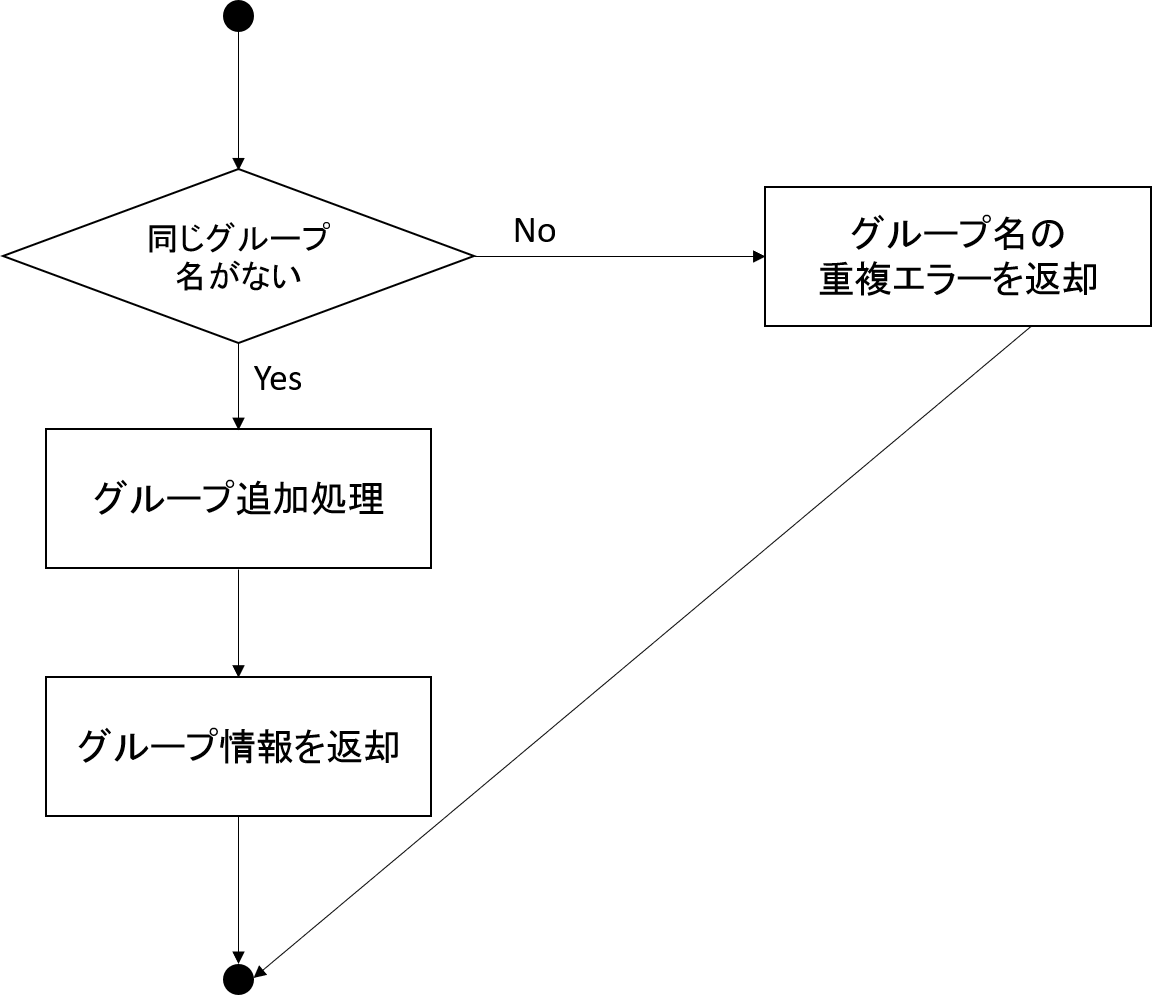
\includegraphics[width=0.75\linewidth,clip]{./img/create_group/sub3.png}
    \caption{[3]のフローチャート}\label{fig:creategroupflow1}
  \end{center}
\end{figure}

\newpage
\subsection{グループ参加システム}
グループ参加システムのシーケンス図とフローチャートを以下に示します。

\begin{figure}[htbp]
  \begin{center}
    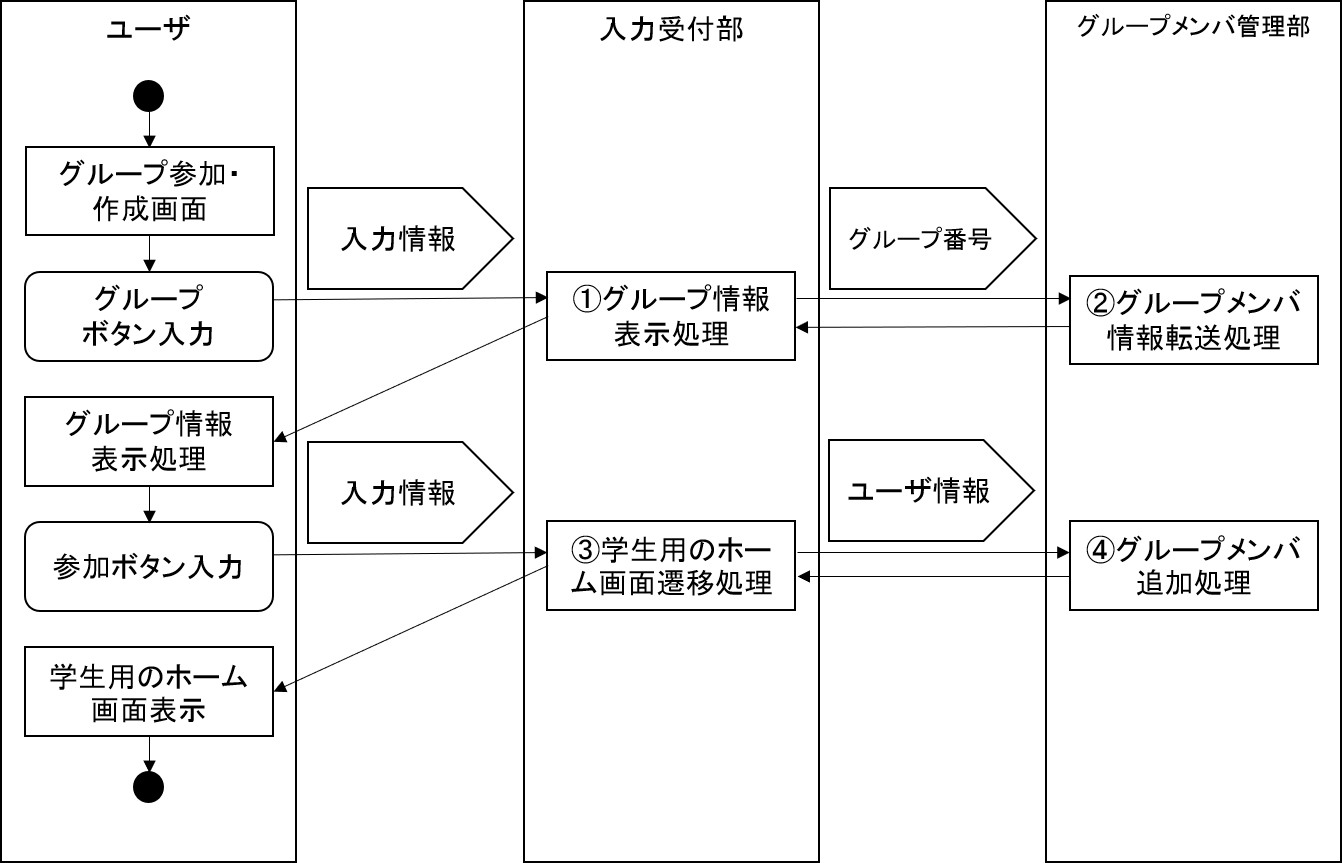
\includegraphics[width=1\linewidth,clip]{./img/join_group/main.png}
    \caption{グループ参加システムのシーケンス図}\label{fig:joingroupseaquence}
  \end{center}
\end{figure}

\begin{figure}[htbp]
 \begin{minipage}{0.5\hsize}
  \begin{center}
   \includegraphics[width=0.5\linewidth,clip]{./img/join_group/sub1.png}
  \end{center}
 \end{minipage}
 \begin{minipage}{0.5\hsize}
  \begin{center}
   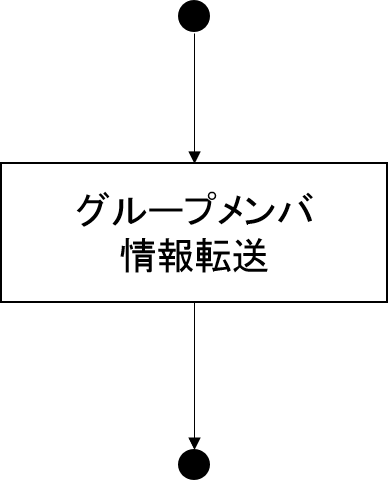
\includegraphics[width=0.5\linewidth,clip]{./img/join_group/sub2.png}
  \end{center}
 \end{minipage}
 \caption{左:[1]のフローチャート 右:[2]のフローチャート}\label{fig:joingroupflow0}
\end{figure}

\begin{figure}[htbp]
 \begin{minipage}{0.5\hsize}
  \begin{center}
   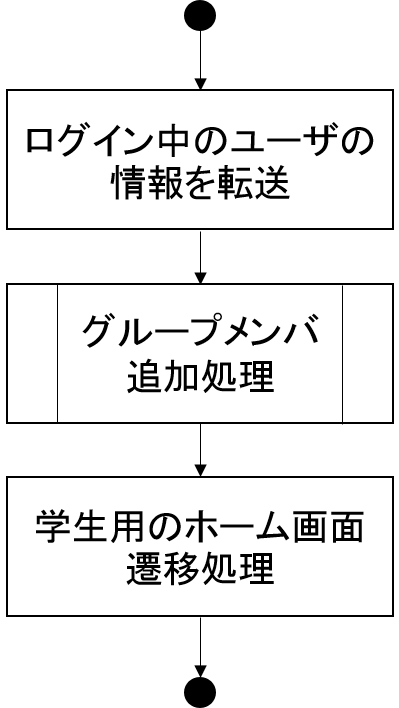
\includegraphics[width=0.5\linewidth,clip]{./img/join_group/sub3.png}
  \end{center}
 \end{minipage}
 \begin{minipage}{0.5\hsize}
  \begin{center}
   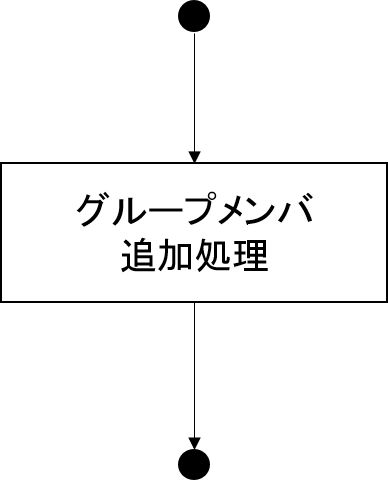
\includegraphics[width=0.5\linewidth,clip]{./img/join_group/sub4.png}
  \end{center}
 \end{minipage}
 \caption{左:[3]のフローチャート 右:[4]のフローチャート}\label{fig:joingroupflow0}
\end{figure}



\newpage
\subsection{グループ編集システム}
グループ編集システムのシーケンス図とフローチャートを以下に示します。

\begin{figure}[htbp]
  \begin{center}
    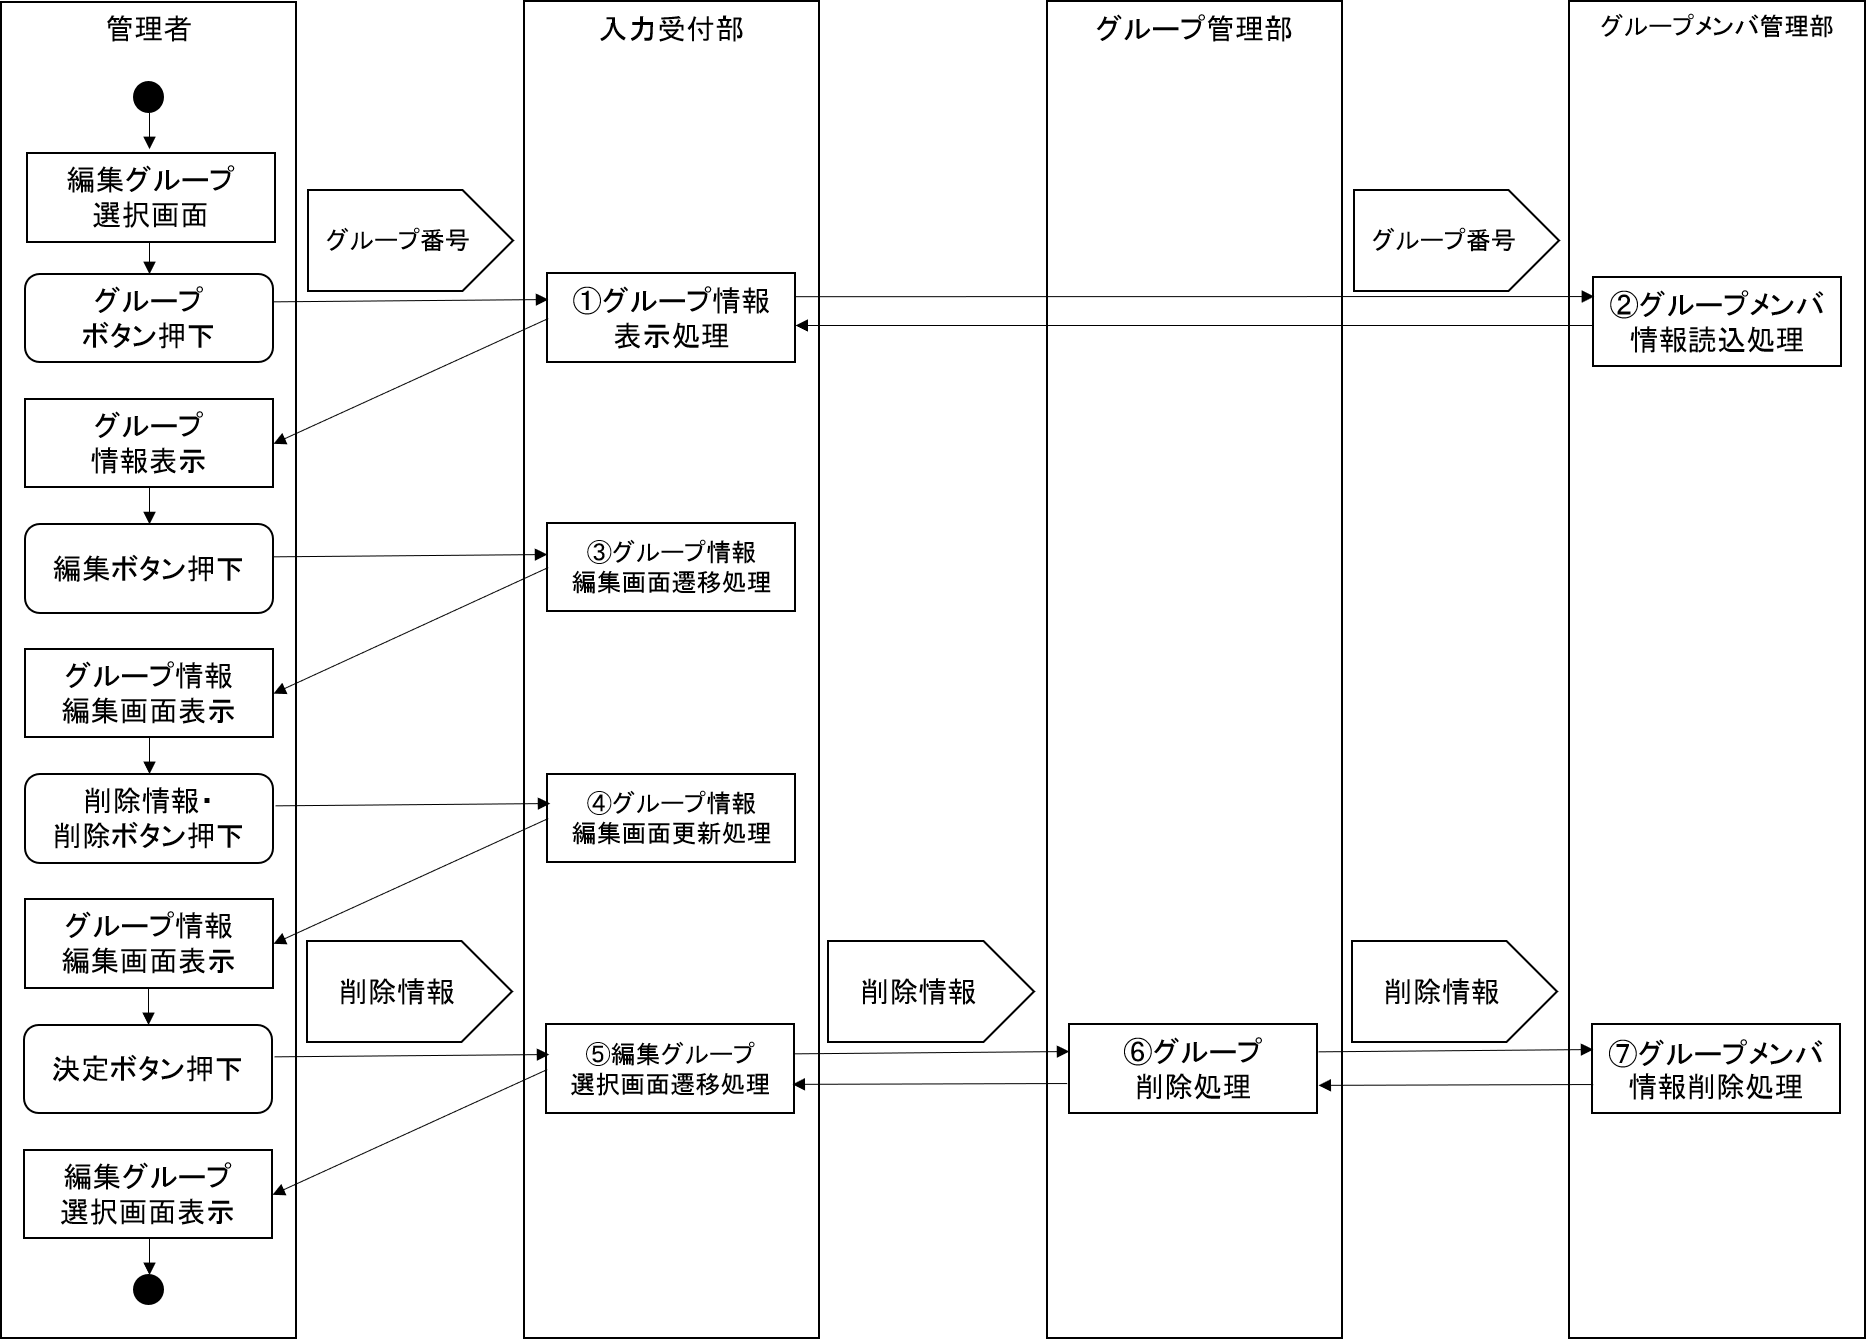
\includegraphics[width=1\linewidth,clip]{./img/edit_group/main.png}
    \caption{グループ編集システムのシーケンス図}\label{fig:editgroupseaquence}
  \end{center}
\end{figure}

\begin{figure}[htbp]
 \begin{minipage}{0.5\hsize}
  \begin{center}
   \includegraphics[width=0.45\linewidth,clip]{./img/edit_group/sub1.png}
  \end{center}
 \end{minipage}
 \begin{minipage}{0.5\hsize}
  \begin{center}
   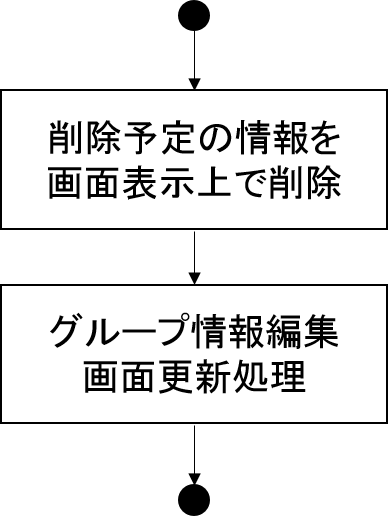
\includegraphics[width=0.45\linewidth,clip]{./img/edit_group/sub2.png}
  \end{center}
 \end{minipage}
 \caption{左:[1]のフローチャート 右:[2]のフローチャート}\label{fig:editgroupflow0}
\end{figure}

\begin{figure}[htbp]
 \begin{minipage}{0.5\hsize}
  \begin{center}
   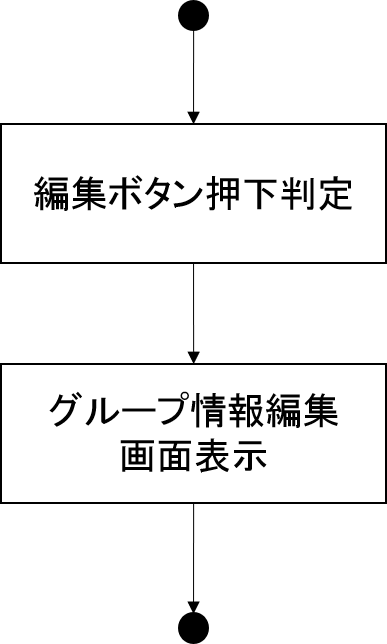
\includegraphics[width=0.45\linewidth,clip]{./img/edit_group/sub3.png}
  \end{center}
 \end{minipage}
 \begin{minipage}{0.5\hsize}
  \begin{center}
   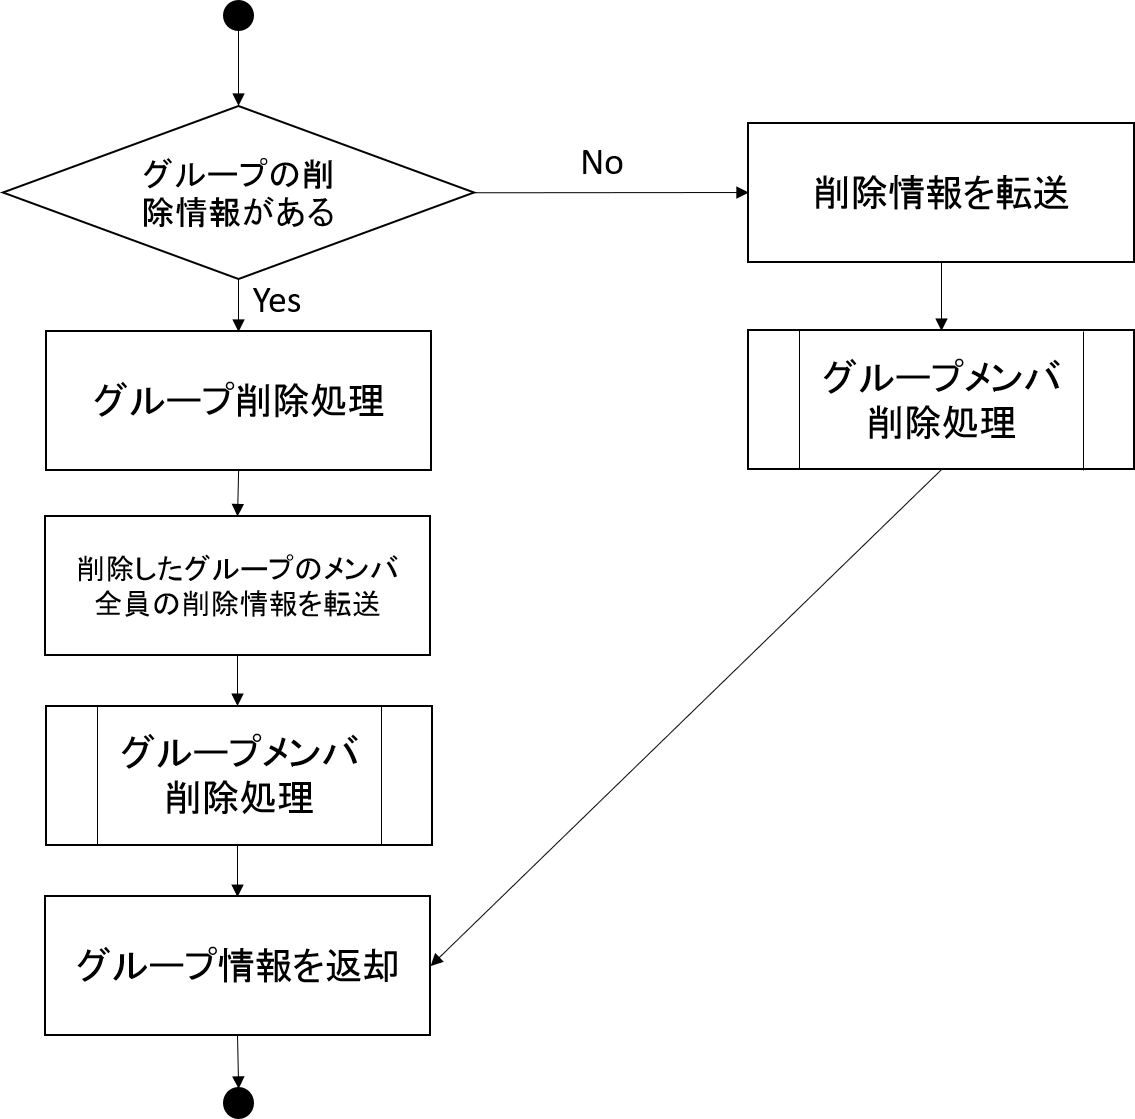
\includegraphics[width=1.2\linewidth,clip]{./img/edit_group/sub4.png}
  \end{center}
 \end{minipage}
 \caption{左:[3]のフローチャート 右:[4]のフローチャート}\label{fig:editgroupflow0}
\end{figure}

\begin{figure}[htbp]
  \begin{center}
    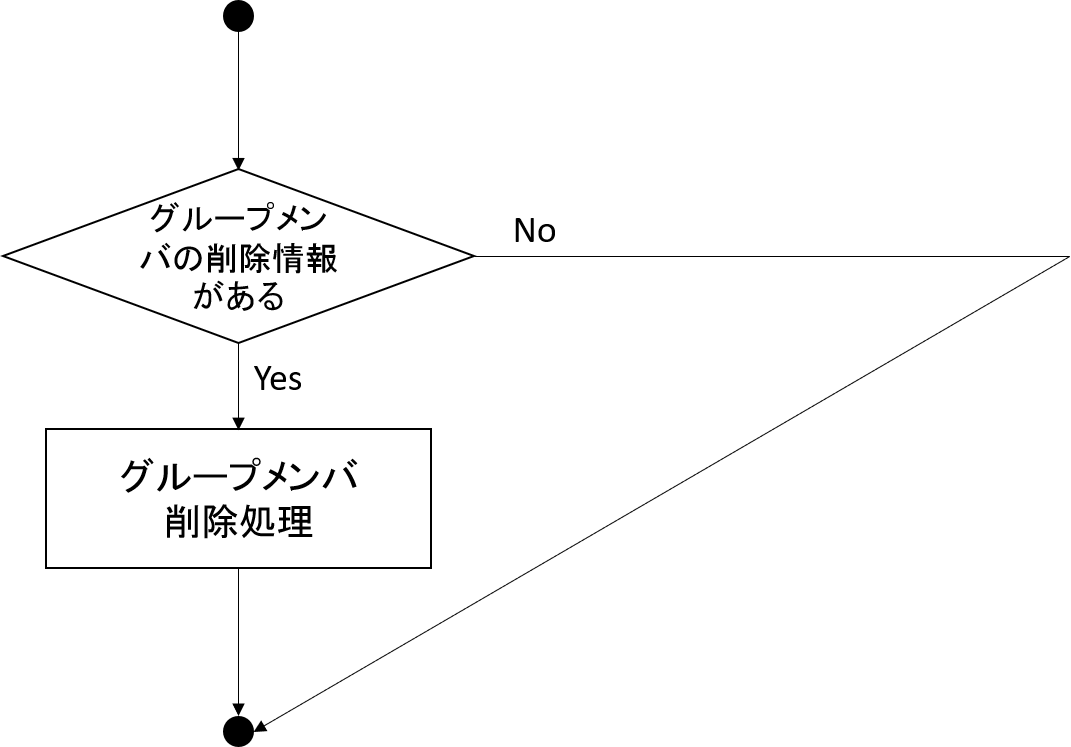
\includegraphics[width=0.5\linewidth,clip]{./img/edit_group/sub5.png}
    \caption{[5]のフローチャート}\label{fig:editgroupflow1}
  \end{center}
\end{figure}


\newpage
\subsection{授業作成・編集システム}
授業作成システムのシーケンス図とフローチャートを以下に示します。

\begin{figure}[htbp]
  \begin{center}
    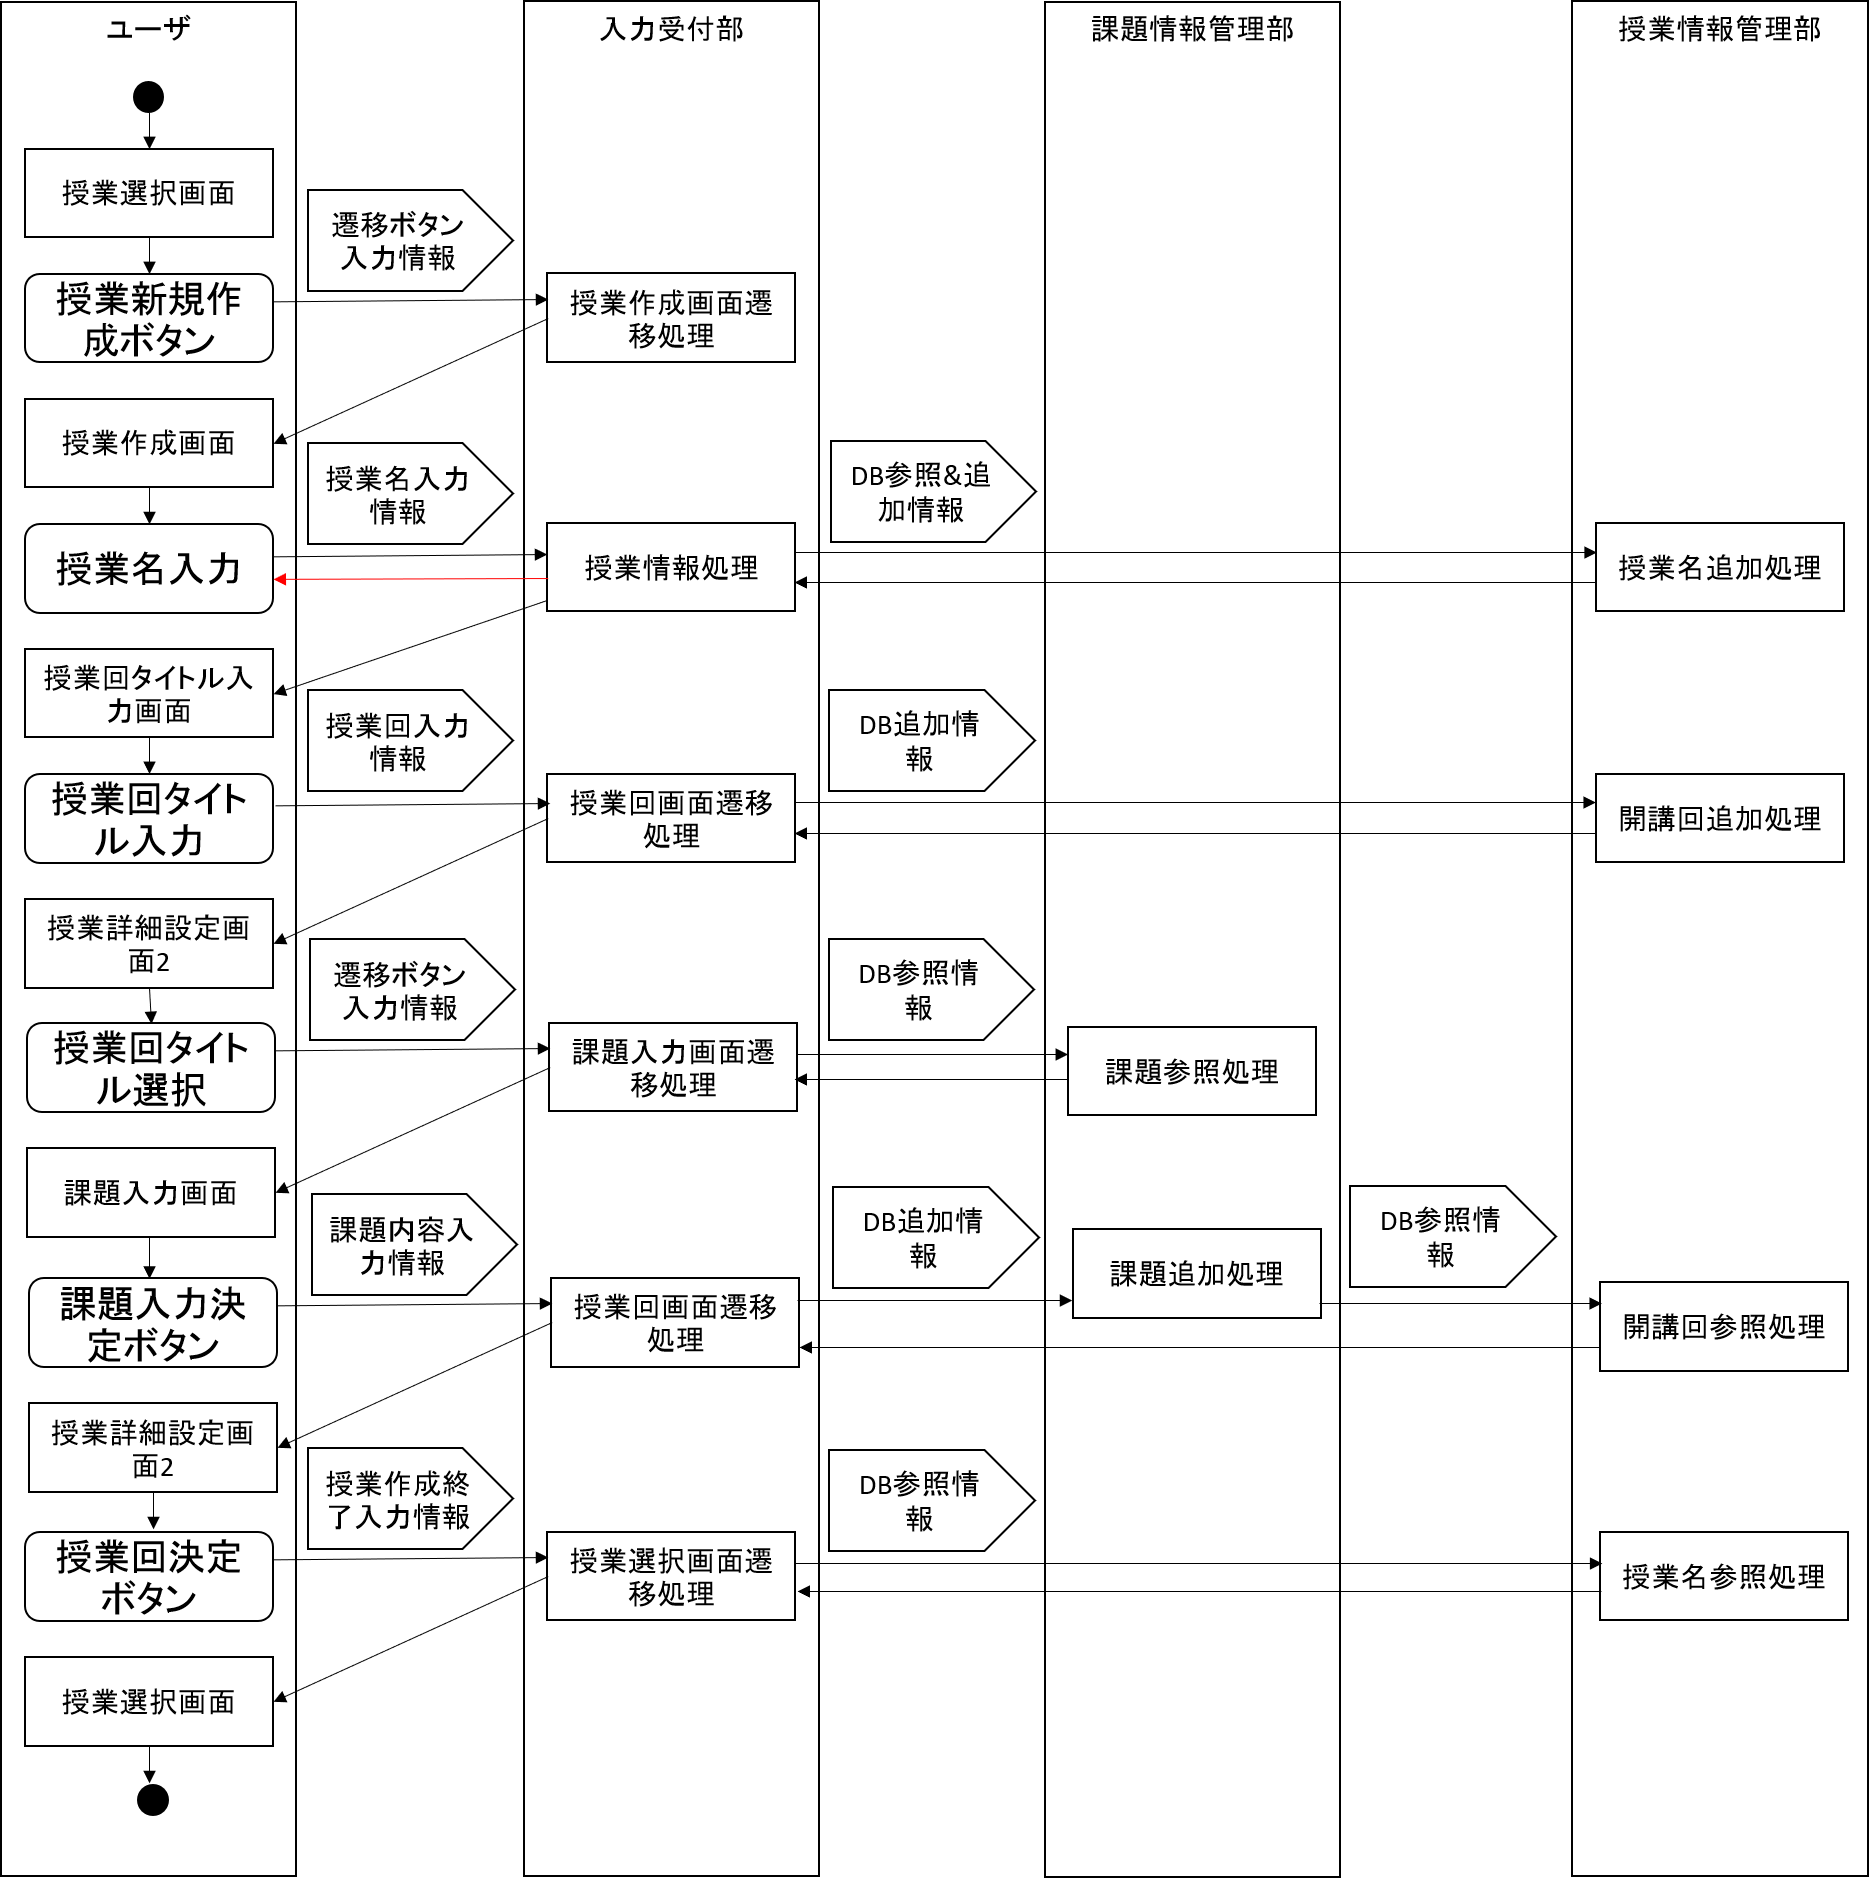
\includegraphics[width=1\linewidth,clip]{./img/create_lecture/main.png}
    \caption{授業作成システムのシーケンス図}\label{fig:createlectureseaquence}
  \end{center}
\end{figure}

\begin{figure}[htbp]
 \begin{minipage}{0.5\hsize}
  \begin{center}
   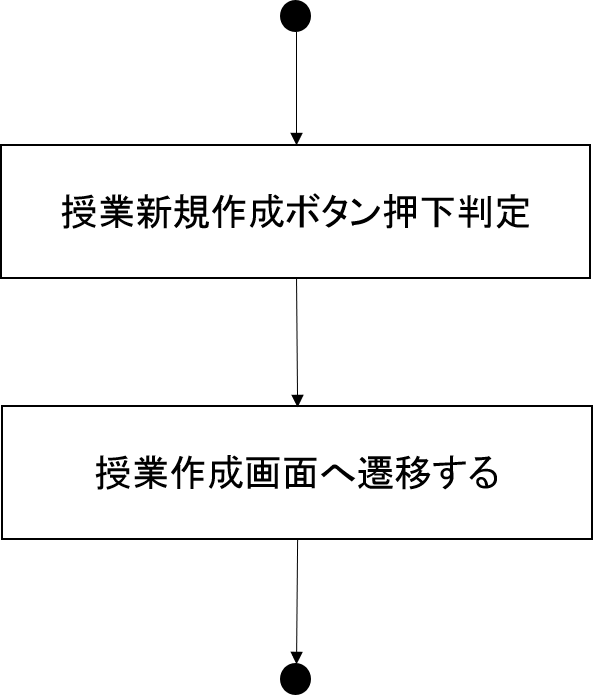
\includegraphics[width=0.5\linewidth,clip]{./img/create_lecture/sub1.png}
  \end{center}
 \end{minipage}
 \begin{minipage}{0.5\hsize}
  \begin{center}
   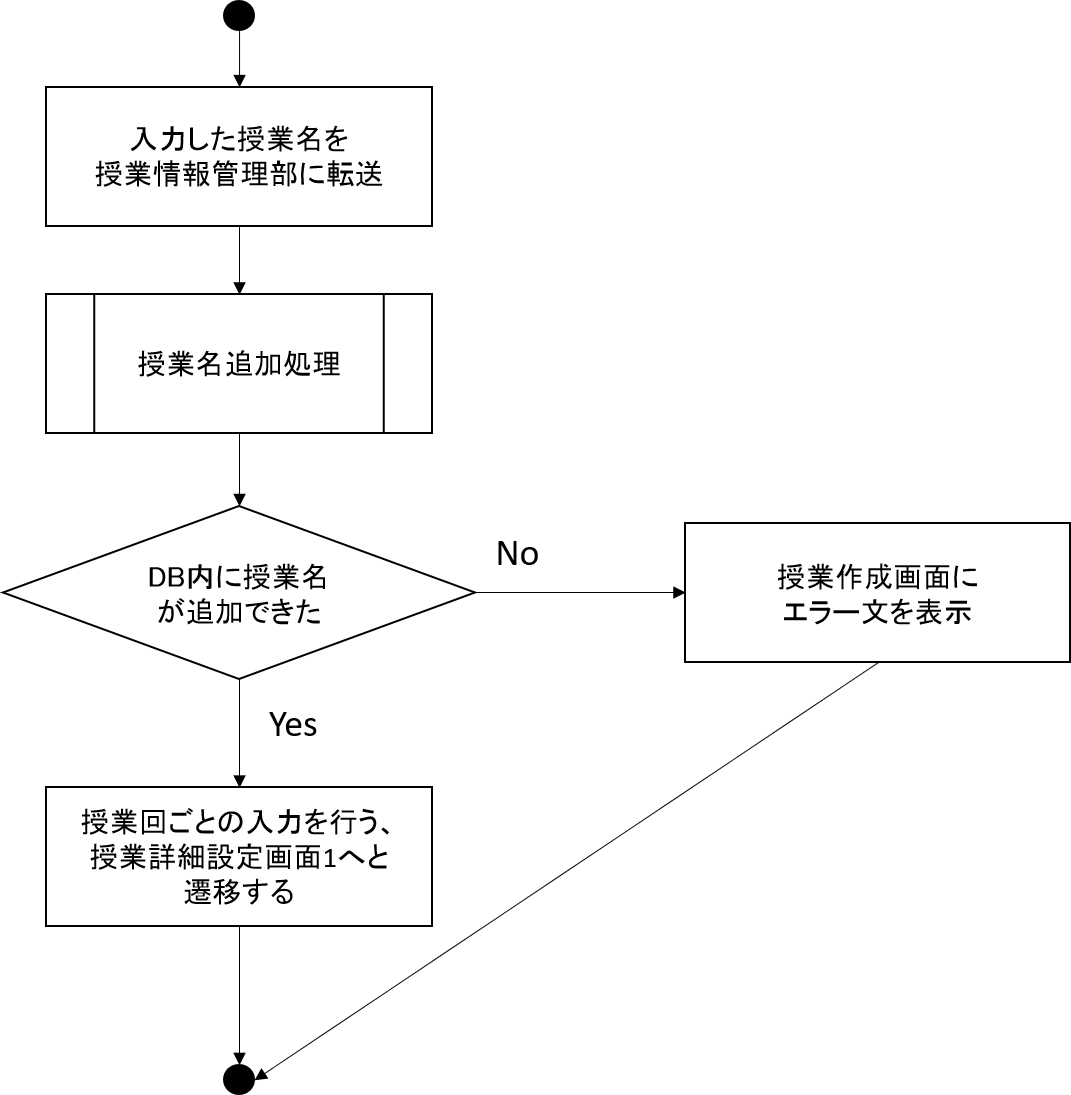
\includegraphics[width=1\linewidth,clip]{./img/create_lecture/sub2.png}
  \end{center}
 \end{minipage}
 \caption{左:[1]のフローチャート 右:[2]のフローチャート}\label{fig:createlectureflow0}
\end{figure}

\begin{figure}[htbp]
 \begin{minipage}{0.5\hsize}
  \begin{center}
   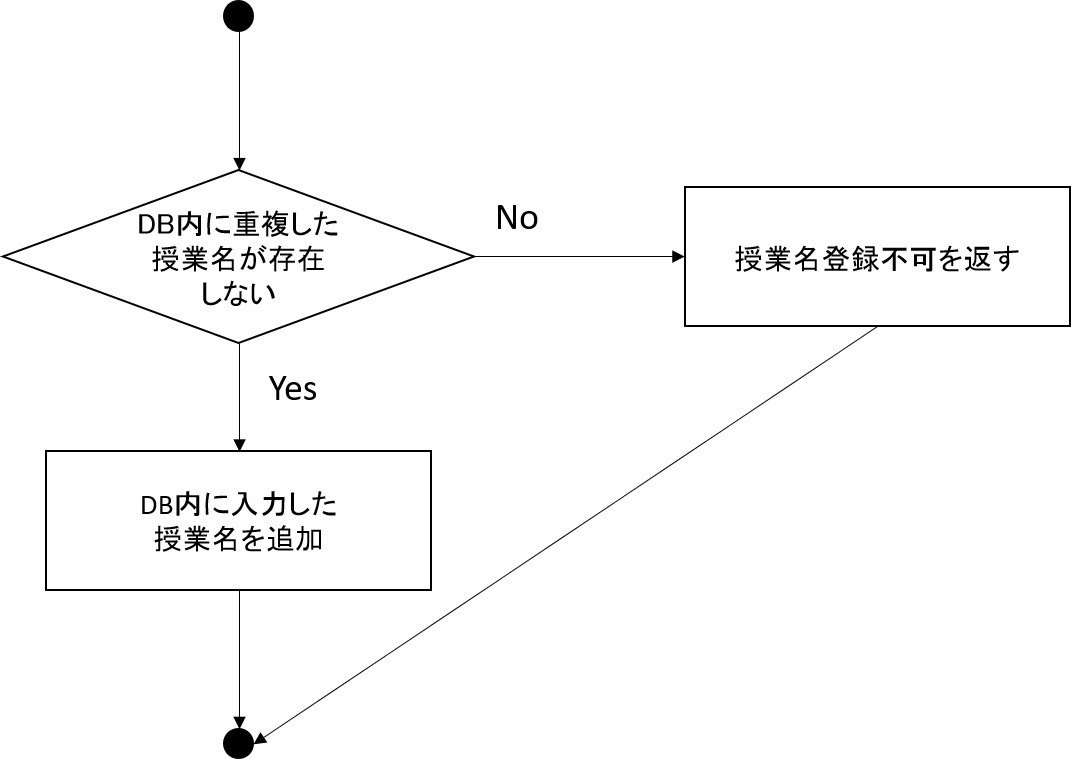
\includegraphics[width=1\linewidth,clip]{./img/create_lecture/sub3.png}
  \end{center}
 \end{minipage}
 \begin{minipage}{0.5\hsize}
  \begin{center}
   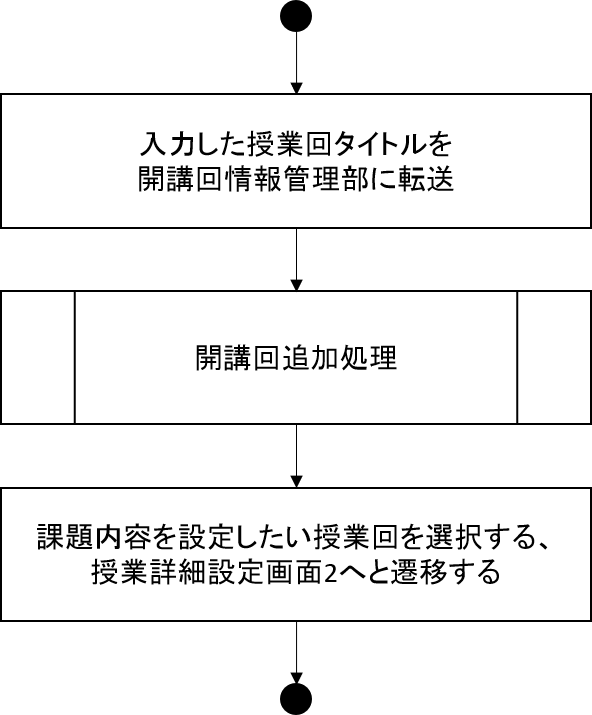
\includegraphics[width=0.5\linewidth,clip]{./img/create_lecture/sub4.png}
  \end{center}
 \end{minipage}
 \caption{左:[3]のフローチャート 右:[4]のフローチャート}\label{fig:createlectureflow1}
\end{figure}

\begin{figure}[htbp]
 \begin{minipage}{0.5\hsize}
  \begin{center}
   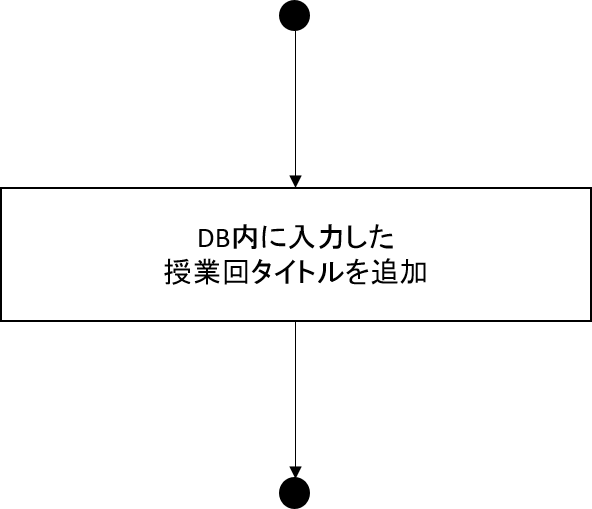
\includegraphics[width=0.5\linewidth,clip]{./img/create_lecture/sub5.png}
  \end{center}
 \end{minipage}
 \begin{minipage}{0.5\hsize}
  \begin{center}
   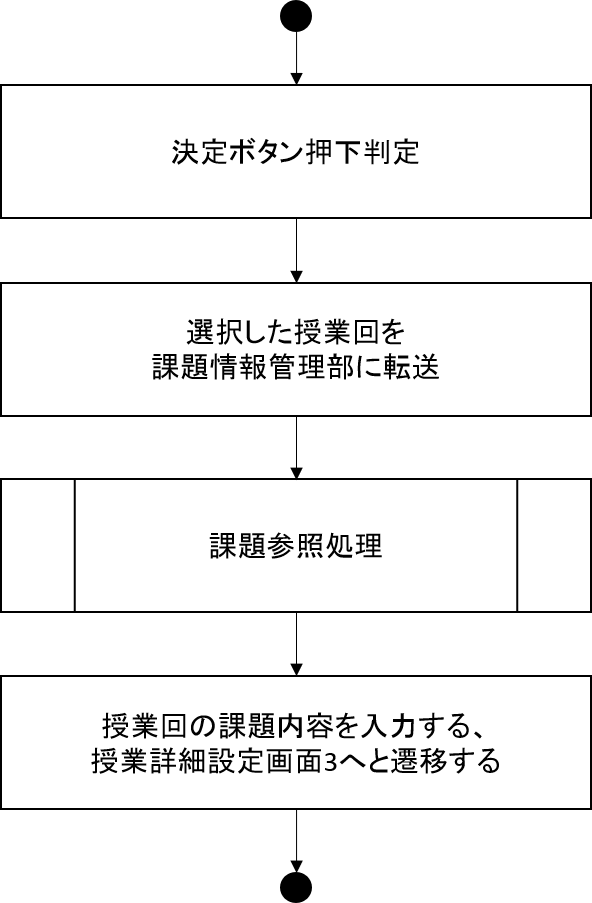
\includegraphics[width=0.5\linewidth,clip]{./img/create_lecture/sub6.png}
  \end{center}
 \end{minipage}
 \caption{左:[5]のフローチャート 右:[6]のフローチャート}\label{fig:createlectureflow2}
\end{figure}

\begin{figure}[htbp]
 \begin{minipage}{0.5\hsize}
  \begin{center}
   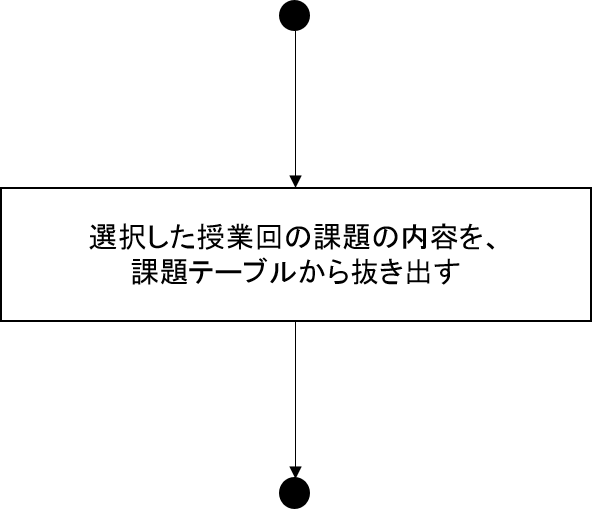
\includegraphics[width=0.5\linewidth,clip]{./img/create_lecture/sub7.png}
  \end{center}
 \end{minipage}
 \begin{minipage}{0.5\hsize}
  \begin{center}
   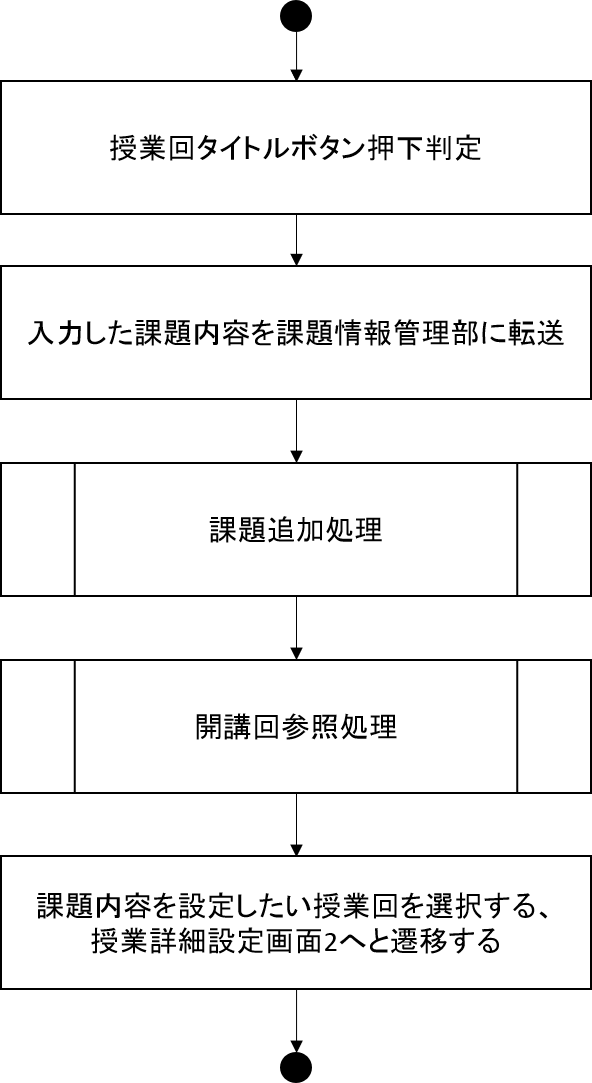
\includegraphics[width=0.5\linewidth,clip]{./img/create_lecture/sub8.png}
  \end{center}
 \end{minipage}
 \caption{左:[7]のフローチャート 右:[8]のフローチャート}\label{fig:createlectureflow3}
\end{figure}

\begin{figure}[htbp]
 \begin{minipage}{0.5\hsize}
  \begin{center}
   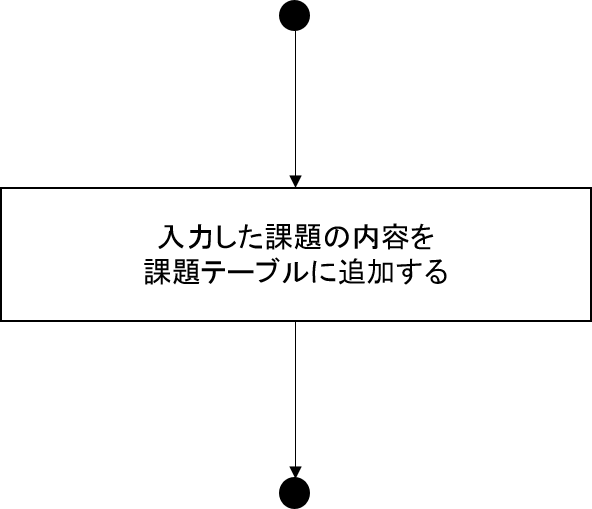
\includegraphics[width=0.5\linewidth,clip]{./img/create_lecture/sub9.png}
  \end{center}
 \end{minipage}
 \begin{minipage}{0.5\hsize}
  \begin{center}
   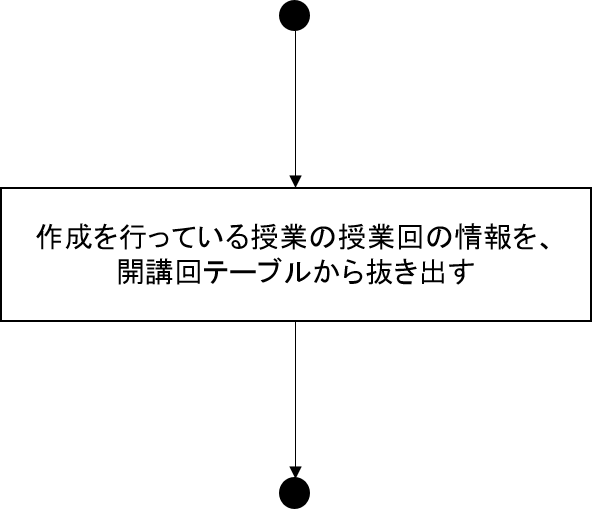
\includegraphics[width=0.5\linewidth,clip]{./img/create_lecture/sub10.png}
  \end{center}
 \end{minipage}
 \caption{左:[9]のフローチャート 右:[10]のフローチャート}\label{fig:createlectureflow4}
\end{figure}

\begin{figure}[htbp]
 \begin{minipage}{0.5\hsize}
  \begin{center}
   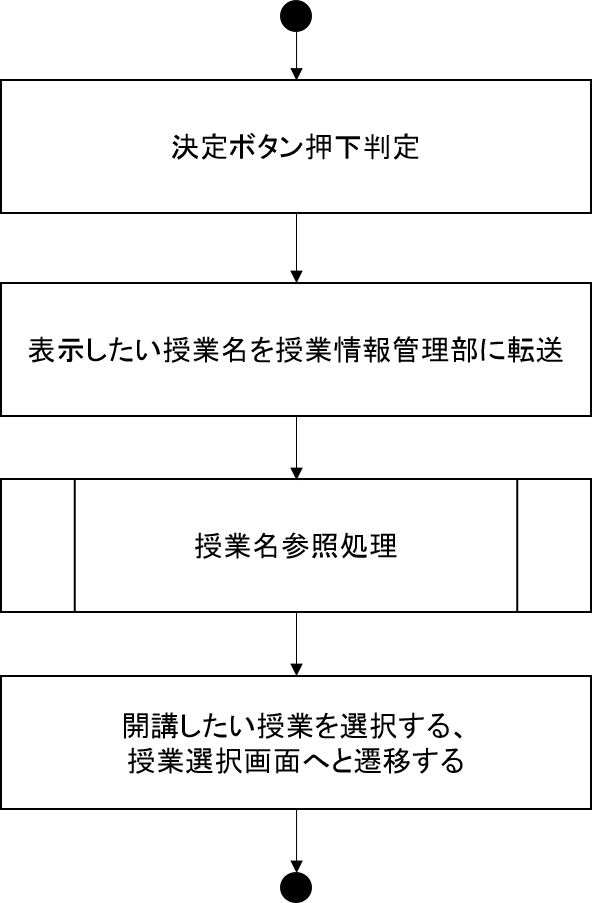
\includegraphics[width=0.5\linewidth,clip]{./img/create_lecture/sub11.png}
  \end{center}
 \end{minipage}
 \begin{minipage}{0.5\hsize}
  \begin{center}
   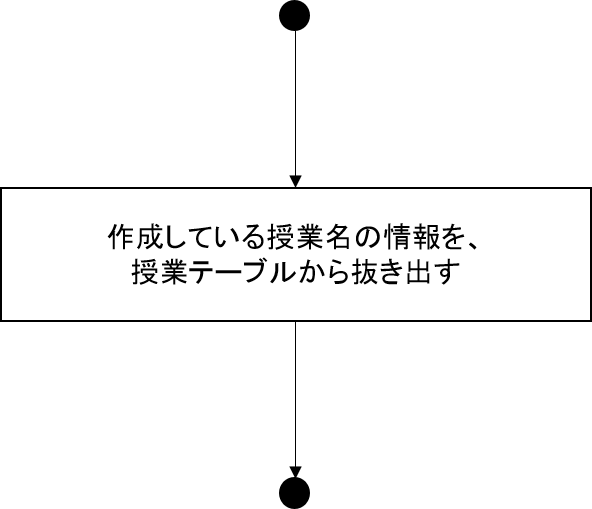
\includegraphics[width=0.5\linewidth,clip]{./img/create_lecture/sub12.png}
  \end{center}
 \end{minipage}
 \caption{左:[11]のフローチャート 右:[12]のフローチャート}\label{fig:createlectureflow5}
\end{figure}


\newpage
\subsection{授業引き継ぎシステム}
授業引き継ぎシステムのシーケンス図とフローチャートを以下に示します。

\begin{figure}[htbp]
  \begin{center}
    \includegraphics[width=1\linewidth,clip]{./img/takeover_lecture/main.png}
    \caption{授業引き継ぎシステムのシーケンス図}\label{fig:takeoverlectureseaquence}
  \end{center}
\end{figure}

\begin{figure}[htbp]
 \begin{minipage}{0.5\hsize}
  \begin{center}
   \includegraphics[width=0.45\linewidth,clip]{./img/takeover_lecture/sub1.png}
  \end{center}
 \end{minipage}
 \begin{minipage}{0.5\hsize}
  \begin{center}
   \includegraphics[width=0.45\linewidth,clip]{./img/takeover_lecture/sub2.png}
  \end{center}
 \end{minipage}
 \caption{左:[1]のフローチャート 右:[2]のフローチャート}\label{fig:takeoverlectureflow0}
\end{figure}


\begin{figure}[htbp]
  \begin{center}
    \includegraphics[width=0.5\linewidth,clip]{./img/takeover_lecture/sub3.png}
    \caption{[3]のフローチャート}\label{fig:takeoverflow1.1}
  \end{center}
\end{figure}

\begin{figure}[htbp]
  \begin{center}
    \includegraphics[width=0.5\linewidth,clip]{./img/takeover_lecture/sub4.png}
    \caption{[4]のフローチャート}\label{fig:takeoverflow1.2}
  \end{center}
\end{figure}



\begin{figure}[htbp]
 \begin{minipage}{0.5\hsize}
  \begin{center}
   \includegraphics[width=0.45\linewidth,clip]{./img/takeover_lecture/sub5.png}
  \end{center}
 \end{minipage}
 \begin{minipage}{0.5\hsize}
  \begin{center}
   \includegraphics[width=0.45\linewidth,clip]{./img/takeover_lecture/sub6.png}
  \end{center}
 \end{minipage}
 \caption{左:[5]のフローチャート 右:[6]のフローチャート}\label{fig:takeoverlectureflow2}
\end{figure}

\begin{figure}[htbp]
 \begin{minipage}{0.5\hsize}
  \begin{center}
   \includegraphics[width=0.45\linewidth,clip]{./img/takeover_lecture/sub7.png}
  \end{center}
 \end{minipage}
 \begin{minipage}{0.5\hsize}
  \begin{center}
   \includegraphics[width=0.45\linewidth,clip]{./img/takeover_lecture/sub8.png}
  \end{center}
 \end{minipage}
 \caption{左:[7]のフローチャート 右:[8]のフローチャート}\label{fig:takeoverlectureflow3}
\end{figure}

\begin{figure}[htbp]
 \begin{minipage}{0.5\hsize}
  \begin{center}
   \includegraphics[width=0.45\linewidth,clip]{./img/takeover_lecture/sub9.png}
  \end{center}
 \end{minipage}
 \begin{minipage}{0.5\hsize}
  \begin{center}
   \includegraphics[width=0.45\linewidth,clip]{./img/takeover_lecture/sub10.png}
  \end{center}
 \end{minipage}
 \caption{左:[9]のフローチャート 右:[10]のフローチャート}\label{fig:takeoverlectureflow4}
\end{figure}

\begin{figure}[htbp]
 \begin{minipage}{0.5\hsize}
  \begin{center}
   \includegraphics[width=0.45\linewidth,clip]{./img/takeover_lecture/sub11.png}
  \end{center}
 \end{minipage}
 \begin{minipage}{0.5\hsize}
  \begin{center}
   \includegraphics[width=0.45\linewidth,clip]{./img/takeover_lecture/sub12.png}
  \end{center}
 \end{minipage}
 \caption{左:[11]のフローチャート 右:[12]のフローチャート}\label{fig:takeoverlectureflow5}
\end{figure}

\begin{figure}[htbp]
 \begin{minipage}{0.5\hsize}
  \begin{center}
   \includegraphics[width=0.45\linewidth,clip]{./img/takeover_lecture/sub13.png}
  \end{center}
 \end{minipage}
 \begin{minipage}{0.5\hsize}
  \begin{center}
   \includegraphics[width=0.45\linewidth,clip]{./img/takeover_lecture/sub14.png}
  \end{center}
 \end{minipage}
 \caption{左:[13]のフローチャート 右:[14]のフローチャート}\label{fig:takeoverlectureflow6}
\end{figure}


\newpage
\subsection{進捗確認システム}
進捗確認システムのシーケンス図とフローチャートを以下に示します。

\begin{figure}[htbp]
  \begin{center}
    \includegraphics[width=1\linewidth,clip]{./img/preg_check/main.png}
    \caption{進捗確認システムのシーケンス図}\label{fig:preg_checkseaquence}
  \end{center}
\end{figure}

\begin{figure}[htbp]
 \begin{minipage}{0.5\hsize}
  \begin{center}
   \includegraphics[width=0.45\linewidth,clip]{./img/preg_check/sub1.png}
  \end{center}
 \end{minipage}
 \begin{minipage}{0.5\hsize}
  \begin{center}
   \includegraphics[width=0.45\linewidth,clip]{./img/preg_check/sub2.png}
  \end{center}
 \end{minipage}
 \caption{左:[1]のフローチャート 右:[2]のフローチャート}\label{fig:pregcheckflow0}
\end{figure}

\begin{figure}[htbp]
  \begin{center}
    \includegraphics[width=0.3\linewidth,clip]{./img/preg_check/sub3.png}
    \caption{[3]のフローチャート}\label{fig:pregcheckflow1}
  \end{center}
\end{figure}

\newpage
\subsection{質問閲覧システム}
質問閲覧システムのシーケンス図とフローチャートを以下に示します。

\begin{figure}[htbp]
  \begin{center}
    \includegraphics[width=1\linewidth,clip]{./img/q_read/main.png}
    \caption{質問閲覧システムのシーケンス図}\label{fig:qreadseaquence}
  \end{center}
\end{figure}

\begin{figure}[htbp]
 \begin{minipage}{0.5\hsize}
  \begin{center}
   \includegraphics[width=0.45\linewidth,clip]{./img/q_read/sub1.png}
  \end{center}
 \end{minipage}
 \begin{minipage}{0.5\hsize}
  \begin{center}
   \includegraphics[width=0.45\linewidth,clip]{./img/q_read/sub2.png}
  \end{center}
 \end{minipage}
 \caption{左:[1]のフローチャート 右:[2]のフローチャート}\label{fig:qreadflow0}
\end{figure}

\newpage
\subsection{過去の質問閲覧システム}
過去の質問閲覧システムのシーケンス図とフローチャートを以下に示します。

\begin{figure}[htbp]
  \begin{center}
    \includegraphics[width=1\linewidth,clip]{./img/q_read_old/main.png}
    \caption{過去の質問閲覧システムのシーケンス図}\label{fig:qreadoldseaquence}
  \end{center}
\end{figure}

\begin{figure}[htbp]
 \begin{minipage}{0.5\hsize}
  \begin{center}
   \includegraphics[width=0.45\linewidth,clip]{./img/q_read_old/sub1.png}
  \end{center}
 \end{minipage}
 \begin{minipage}{0.5\hsize}
  \begin{center}
   \includegraphics[width=0.45\linewidth,clip]{./img/q_read_old/sub2.png}
  \end{center}
 \end{minipage}
 \caption{左:[1]のフローチャート 右:[2]のフローチャート}\label{fig:qreadoldflow0}
\end{figure}

\begin{figure}[htbp]
 \begin{minipage}{0.5\hsize}
  \begin{center}
   \includegraphics[width=0.45\linewidth,clip]{./img/q_read_old/sub3.png}
  \end{center}
 \end{minipage}
 \begin{minipage}{0.5\hsize}
  \begin{center}
   \includegraphics[width=0.45\linewidth,clip]{./img/q_read_old/sub4.png}
  \end{center}
 \end{minipage}
 \caption{左:[3]のフローチャート 右:[4]のフローチャート}\label{fig:qreadoldflow0}
\end{figure}


\newpage
\subsection{質問送信システム}
質問送信システムのシーケンス図とフローチャートを以下に示します。

\begin{figure}[htbp]
  \begin{center}
    \includegraphics[width=1\linewidth,clip]{./img/q_send/main.png}
    \caption{質問送信システムのシーケンス図}\label{fig:qsendseaquence}
  \end{center}
\end{figure}

\begin{figure}[htbp]
  \begin{center}
    \includegraphics[width=0.3\linewidth,clip]{./img/q_send/sub1.png}
    \caption{[1]のフローチャート}\label{fig:qsendflow0}
  \end{center}
\end{figure}

\begin{figure}[htbp]
 \begin{minipage}{0.5\hsize}
  \begin{center}
   \includegraphics[width=1.2\linewidth,clip]{./img/q_send/sub2.png}
  \end{center}
 \end{minipage}
 \begin{minipage}{0.5\hsize}
  \begin{center}
   \includegraphics[width=0.45\linewidth,clip]{./img/q_send/sub3.png}
  \end{center}
 \end{minipage}
 \caption{左:[2]のフローチャート 右:[3]のフローチャート}\label{fig:qsendflow0}
\end{figure}


\newpage
\subsection{質問回答システム}
質問回答システムのシーケンス図とフローチャートを以下に示します。

\begin{figure}[htbp]
  \begin{center}
    \includegraphics[width=1\linewidth,clip]{./img/q_reply/main1.png}
    \caption{質問回答システムのシーケンス図1}\label{fig:qreplyseaquence1}
  \end{center}
\end{figure}

\begin{figure}[htbp]
  \begin{center}
    \includegraphics[width=1\linewidth,clip]{./img/q_reply/main2.png}
    \caption{質問回答システムのシーケンス図2}\label{fig:qreplyseaquence}
  \end{center}
\end{figure}

\begin{figure}[htbp]
  \begin{center}
    \includegraphics[width=0.4\linewidth,clip]{./img/q_reply/sub1.png}
    \caption{[1]のフローチャート}\label{fig:qreplyflow0}
  \end{center}
\end{figure}

\begin{figure}[htbp]
 \begin{minipage}{0.5\hsize}
  \begin{center}
   \includegraphics[width=0.45\linewidth,clip]{./img/q_reply/sub2.png}
  \end{center}
 \end{minipage}
 \begin{minipage}{0.5\hsize}
  \begin{center}
   \includegraphics[width=0.45\linewidth,clip]{./img/q_reply/sub3.png}
  \end{center}
 \end{minipage}
 \caption{左:[2]のフローチャート 右:[3]のフローチャート}\label{fig:qreplyflow1}
\end{figure}


\newpage
\subsection{質問編集システム}
質問編集システムのシーケンス図とフローチャートを以下に示します。

\begin{figure}[htbp]
  \begin{center}
    \includegraphics[width=0.4\linewidth,clip]{./img/q_edit/main.png}
    \caption{質問編集システムのシーケンス図1}\label{fig:qeditseaquence}
  \end{center}
\end{figure}

\begin{figure}[htbp]
 \begin{minipage}{0.5\hsize}
  \begin{center}
   \includegraphics[width=0.45\linewidth,clip]{./img/q_edit/sub1.png}
  \end{center}
 \end{minipage}
 \begin{minipage}{0.5\hsize}
  \begin{center}
   \includegraphics[width=0.45\linewidth,clip]{./img/q_edit/sub2.png}
  \end{center}
 \end{minipage}
 \caption{左:[2]のフローチャート 右:[3]のフローチャート}\label{fig:qeditflow0}
\end{figure}


\newpage
\subsection{質問削除システム}
質問削除システムのシーケンス図とフローチャートを以下に示します。

\begin{figure}[htbp]
  \begin{center}
    \includegraphics[width=1\linewidth,clip]{./img/q_delete/main.png}
    \caption{質問削除システムのシーケンス図}\label{fig:qdeleteseaquence}
  \end{center}
\end{figure}

\begin{figure}[htbp]
  \begin{center}
    \includegraphics[width=0.4\linewidth,clip]{./img/q_delete/sub1.png}
    \caption{[1]のフローチャート}\label{fig:qdeleteflow0}
  \end{center}
\end{figure}

\newpage
